%%%%%%%%%%%%%%
%% Run LaTeX on this file several times to get Table of Contents,
%% cross-references, and citations.

%% If you have font problems, you may edit the w-bookps.sty file
%% to customize the font names to match those on your system.

%% w-bksamp.tex. Current Version: Feb 16, 2012
%%%%%%%%%%%%%%%%%%%%%%%%%%%%%%%%%%%%%%%%%%%%%%%%%%%%%%%%%%%%%%%%
%
%  Sample file for
%  Wiley Book Style, Design No.: SD 001B, 7x10
%  Wiley Book Style, Design No.: SD 004B, 6x9
%
%
%  Prepared by Amy Hendrickson, TeXnology Inc.
%  http://www.texnology.com
%%%%%%%%%%%%%%%%%%%%%%%%%%%%%%%%%%%%%%%%%%%%%%%%%%%%%%%%%%%%%%%%

%%%%%%%%%%%%%
% 7x10
%\documentclass{wileySev}

% 6x9
\documentclass{wileySix}

\usepackage{graphicx}
\usepackage{listings}
\usepackage{float}
\usepackage[urlcolor=blue, colorlinks=true]{hyperref}
\usepackage{color}
\usepackage{textcomp}

\definecolor{codegreen}{rgb}{0,0.6,0}
\definecolor{codegray}{rgb}{0.5,0.5,0.5}
\definecolor{codepurple}{rgb}{0.58,0,0.82}
\definecolor{backcolour}{rgb}{0.95,0.95,0.92}

\lstdefinestyle{mystyle}{
    backgroundcolor=\color{backcolour},
    commentstyle=\color{codegreen},
    keywordstyle=\color{magenta},
    numberstyle=\tiny\color{codegray},
    stringstyle=\color{codepurple},
    basicstyle=\footnotesize,
    breakatwhitespace=false,
    breaklines=true,
    captionpos=b,
    keepspaces=true,
    numbers=left,
    numbersep=5pt,
    showspaces=false,
    showstringspaces=false,
    showtabs=false,
    tabsize=2,
    language=sh
}

\lstset{style=mystyle}

%%%%%%%
%% for times math: However, this package disables bold math (!)
%% \mathbf{x} will still work, but you will not have bold math
%% in section heads or chapter titles. If you don't use math
%% in those environments, mathptmx might be a good choice.

% \usepackage{mathptmx}

% For PostScript text
\usepackage{w-bookps}

%%%%%%%%%%%%%%%%%%%%%%%%%%%%%%%%%%%%%%%%%%%%%%%%%%%%%%%%%%%%%%%%
%% Other packages you might want to use:

% for chapter bibliography made with BibTeX
% \usepackage{chapterbib}

% for multiple indices
% \usepackage{multind}

% for answers to problems
% \usepackage{answers}

%%%%%%%%%%%%%%%%%%%%%%%%%%%%%%
%% Change options here if you want:
%%
%% How many levels of section head would you like numbered?
%% 0= no section numbers, 1= section, 2= subsection, 3= subsubsection
%%==>>
\setcounter{secnumdepth}{3}

%% How many levels of section head would you like to appear in the
%% Table of Contents?
%% 0= chapter titles, 1= section titles, 2= subsection titles,
%% 3= subsubsection titles.
%%==>>
\setcounter{tocdepth}{2}

%% Cropmarks? good for final page makeup
%% \docropmarks

%%%%%%%%%%%%%%%%%%%%%%%%%%%%%%
%
% DRAFT
%
% Uncomment to get double spacing between lines, current date and time
% printed at bottom of page.
% \draft
% (If you want to keep tables from becoming double spaced also uncomment
% this):
% \renewcommand{\arraystretch}{0.6}
%%%%%%%%%%%%%%%%%%%%%%%%%%%%%%

%%%%%%% Demo of section head containing sample macro:
%% To get a macro to expand correctly in a section head, with upper and
%% lower case math, put the definition and set the box
%% before \begin{document}, so that when it appears in the
%% table of contents it will also work:

\newcommand{\VT}[1]{\ensuremath{{V_{T#1}}}}

%% use a box to expand the macro before we put it into the section head:

\newbox\sectsavebox
\setbox\sectsavebox=\hbox{\boldmath\VT{xyz}}

%%%%%%%%%%%%%%%%% End Demo


\begin{document}


\booktitle{SIG (Sistem Informasi Geografis)}
\subtitle{Semester 5}

\authors{D4TI3A\\
\affil{Angkatan 2017}
%Floyd J. Fowler, Jr.\\
%\affil{University of New Mexico}
}

\offprintinfo{SIG (Sistem Informasi Geografis), First Edition}{D4TI3A}

%% Can use \\ if title, and edition are too wide, ie,
%% \offprintinfo{Survey Methodology,\\ Second Edition}{Robert M. Groves}

%%%%%%%%%%%%%%%%%%%%%%%%%%%%%%
%%
\halftitlepage

%\titlepage


\begin{copyrightpage}{2019}
%Survey Methodology / Robert M. Groves . . . [et al.].
%\       p. cm.---(Wiley series in survey methodology)
%\    ``Wiley-Interscience."
%\    Includes bibliographical references and index.
%\    ISBN 0-471-48348-6 (pbk.)
%\    1. Surveys---Methodology.  2. Social 
%\  sciences---Research---Statistical methods.  I. Groves, Robert M.  II. %
%Series.\\
%
%HA31.2.S873 2007
%001.4'33---dc22                                             2004044064
\end{copyrightpage}

\dedication{`Jika Kamu tidak dapat menahan lelahnya belajar,
Maka kamu harus sanggup menahan perihnya Kebodohan.'
~Imam Syafi'i~}

\begin{contributors}
\name{Rolly Maulana Awangga,} Informatics Research Center., Politeknik Pos Indonesia, Bandung,
Indonesia



\end{contributors}

\contentsinbrief
\tableofcontents
\listoffigures
\listoftables
\lstlistoflistings


\begin{foreword}
Sepatah kata dari Kaprodi, Kabag Kemahasiswaan dan Mahasiswa
\end{foreword}

\begin{preface}
Buku ini diciptakan bagi yang awam dengan flask sekalipun.

\prefaceauthor{R. M. Awangga}
\where{Bandung, Jawa Barat\\
Februari, 2019}
\end{preface}


\begin{acknowledgments}
Terima kasih atas semua masukan dari para mahasiswa agar bisa membuat buku ini 
lebih baik dan lebih mudah dimengerti.

Terima kasih ini juga ditujukan khusus untuk team IRC yang 
telah fokus untuk belajar dan memahami bagaimana buku ini mendampingi proses 
Intership.
\authorinitials{R. M. A.}
\end{acknowledgments}

\begin{acronyms}
\acro{ACGIH}{American Conference of Governmental Industrial Hygienists}
\acro{AEC}{Atomic Energy Commission}
\acro{OSHA}{Occupational Health and Safety Commission}
\acro{SAMA}{Scientific Apparatus Makers Association}
\end{acronyms}

\begin{glossary}
\term{git}Merupakan manajemen sumber kode yang dibuat oleh linus torvald.

\term{bash}Merupakan bahasa sistem operasi berbasiskan *NIX.

\term{linux}Sistem operasi berbasis sumber kode terbuka yang dibuat oleh Linus Torvald
\end{glossary}

\begin{symbols}
\term{A}Amplitude

\term{\hbox{\&}}Propositional logic symbol 

\term{a}Filter Coefficient

\bigskip

\term{\mathcal{B}}Number of Beats
\end{symbols}

\begin{introduction}

%% optional, but if you want to list author:

\introauthor{Rolly Maulana Awangga, S.T., M.T.}
{Informatics Research Center\\
Bandung, Jawa Barat, Indonesia}

Pada era disruptif  \index{disruptif}\index{disruptif!modern} 
saat ini. git merupakan sebuah kebutuhan dalam sebuah organisasi pengembangan perangkat lunak.
Buku ini diharapkan bisa menjadi penghantar para programmer, analis, IT Operation dan Project Manajer.
Dalam melakukan implementasi git pada diri dan organisasinya.

Rumusnya cuman sebagai contoh aja biar keren\cite{awangga2018sampeu}.

\begin{equation}
ABC {\cal DEF} \alpha\beta\Gamma\Delta\sum^{abc}_{def}
\end{equation}

\end{introduction}

%%%%%%%%%%%%%%%%%% Isi Buku %%%%%%%%%%%%%%%%%%
\chapter{Tugas Pertama}
\section{Arjun Yuda Firwanda (1174008)}
\subsection{Pengertian}
Sistem Informasi Geografis merupakan sistem informasi yang secara khusus mengelola data yang memiliki spasial atau keruangan.

Secara ringkasnya sistem informasi geografis merupakan sistem komputer yang memiliki kemampuan untuk membangun, menyimpan, mengelola dan menampilkan informasi bereferensi geografis, contohnya sebuah data yang diidentifikasi menurut lokasinya.

Pengertian Sistem Informasi Geografis merupakan gabungan dari tiga unsur pokok.
\begin{itemize}
	\item Sistem merupakan sekumpulan objek.
	\item Sistem Informasi merupakan sistem antara manusia dan mesin untuk menyajikan informasi untuk mendukung suatu fungsi operasi, manajemen dan pengambilan keputusan.
	\item Geografi  merupakan pengertian yang mengenai tempat-tempat yang terletak di permukaan bumi dan informasi mengenai keterangan dan posisi yang terdapat di permukaan bumi.
\end{itemize}

\subsection{Sejarah}
Awal dikenalnya Sistem Informasi Geografis (Geogragis Informastion System) tidak lepas dari perkembangan dalam bidang teknologi. Pada awal 1960-an perkembangan teknologi digunakan untuk bidang diluar militer. Pada ahli meterologi, geologi dan geofisika mulai menggunakan komputer dalam pembuatan peta.

Tahun 1963 di Kanada muncul CGIS (Canada Geographic Information System) dan selanjutnya menjadi GIS pertama di dunia. Dua tahun kemudian di Amerika Serikat beroperasi sistem bernama MIDAS yang digunakan untuk memproses data-data sumber daya alam.

\subsection{Koordinat}
Sistem Koordinat, osisi suatu titik biasanya dapat dinyatakan dengan koordinat yang mengacu pada suatu sistem koordinat tertentu.

\begin{itemize}
	\item Lokasi Titik Nol dari Sistem Koordinat
Posisi suatu titik di permukaan bumi umumnya ditetapkan dalam/terhadap suatu sistem koordinat terestris. Titik nol dari sistem koordinat terestris ini dapat berlokasi di titik pusat massa bumi (sistem koordinat geosentrik), maupun di salah satu titik di permukaan bumi (sistem koordinat toposentrik).  
	\item Orientasi dari Sumbu-sumbu Koordinat
Posisi tiga-dimensi suatu titik di permukaan bumi umumnya dinyatakan dalam suatu sistem koordinat geosentrik. Tergantung dari parameter-parameter pendefinisi koordinat yang digunakan. Ada dua sistem koordinat yang umum digunakan, yaitu sistem koordinat Kartesian (X,Y,Z) dan sistem koordinat Geodetik (L,B,h).
\end{itemize}


\subsection{Data Geospasial}
Data geospasial adalah kumpulan fakta yang berupa informasi tentang ruang kebumian (geospasial) yang menunjukan lokasi atau posisi dari suatu tempat atau objek yang direpresentasikan pada sebuah garis titik koordinat. Data geospasial dibagi menjadi 2 yaitu:

\begin{enumerate}
	\item Data Vector
Dalam bentuk data vector bagian objek dibumi ditampilkan sebagai kumpulan titik , garis dan polygon dimana sekumpulan tiitik yang saling terhubung akan membentuk garis dan garis yang saling terhubung antara titik awal dan titik akhir dengan nilai koordinat ynag sama akan membentuk polygon . Data vector dibagi menjadi 2 yaitu:

	\begin{itemize}
		\item Culture, memaparkan atau menampilkan data geospasial yang disertai dengan nama atribut atau memberikan keterangan atas nama dari objek di bumi. Contohnya nama dari suatu Negara, indicator batas air (keterangan kedalaman air laut), nama provinsi, daerah, wilayah dsb.
		\item Physical, memaparkan atau menampilkan data geospasial mengenai bentuk fisiknya atau gambaran tentang objek-objek alam yang ada dibumi. Contohnya gambaran laut, garis pantai, terumbu karang, danau dsb.
	\end{itemize}

	\item Data Raster, dapat menampilkan permukaan bumi seperti bentuk aslinya atau seperti dalam peta asli yang terlihat jelas dari setiap objek dengan keadaan alamnya. Data raster dibentuk agar menampilkan objek berupa elemen matriks atau grid, yang merepresentasikan objek dari data geospasial mengenai batas-batas yang berubah, ketinggian tanah.
\end{enumerate}

\subsection{Link}
\href{https://www.youtube.com/watch?v=HGscljVrxrE&feature=youtu.be}{Cek Di Youtubeku}

\subsection{Plagiarism}
\begin{figure}[Cek Plagiat]
	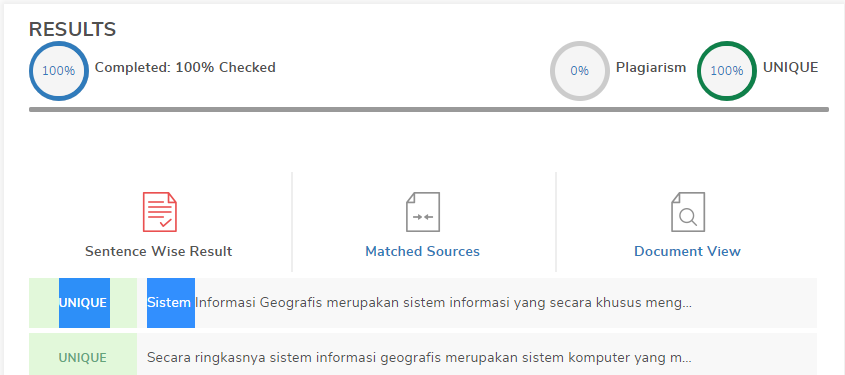
\includegraphics[width=4cm]{figures/1174008/pelagiat.png}
	\centering
	\caption{Cek Plagiat.}
\end{figure}

\section{NAMA (NPM)}
\subsection{Pengertian}
\subsection{Sejarah}
\subsection{Koordinat}
\subsection{Data Geospasial}
\subsection{Link}
\subsection{Plagiarism}

\subsection{Cara Penggunaan}
\subsubsection{Gambar}

\hfill\break

Contoh Gambar
\begin{figure}[H]
	
\includegraphics[width=4cm]{figures/himatif.png}
	\centering
	\caption{Contoh gambar.}
\end{figure}

\subsubsection{List}
\begin{enumerate}
	\item Satu
	\item Dua
\end{enumerate}

\begin{itemize}
	\item Satu
	\item Dua
\end{itemize}

\href{link kamu}{alias}
contoh link
\href{https://www.google.com/}{klik me}
\section{Damara Benedikta (1174012)}
\subsection{Pengertian SIG}
SIG atau system informasi geografis merupakan sebuah system informasi yang berbasis computer dimana dirancang untuk dapat bekerja mengolah data yang memiliki informasi spasial. Didalam system tersebut dapat melakukan pengecekan, pengintegrasian, manipulasi,analisa dan menampilkan data secara spasial yang mereferensikan kondisi bumi

\subsection{Sejarah SIG}
Pada 35000 tahun yang lalu para pemburu diprancis mereka menggambar hewan pemangsa dan juga garis yang dipercya sebagai rute dari migrasi hewan hewan tersebut. Itu merupakan sebuah catatan awal pada system informasi geografis. 
awal abad 20 dimulailah pengembangan litografi foto yang mana peta dipisahakan beberapa lapisan (layer). Perkembangan perangkat keras komputer yang dipacu oleh penelitian senjata nuklir membawa aplikasi pemetaan menjadi multifungsi pada awal tahun 1960-an.
Sehingga pada tahun 1967 sebagai awal pengembangan  dari SIG yang  diterapkan di Ottawa, Ontario oleh Departemen Energi, Pertambangan dan Sumber Daya. SIG sendiri dikembangkan oleh Roger Tomlinson, yang kemudian disebut CGIS (Canadian GIS – SIG Kanada), yang memiliki kegunaan sebagai penympanan penganalisa dan pengolahan data yang telah dikumpulkan untuk inventarisasi tanah di Kanada.
Canadian GIS adalah system pertama yang berasal dari perbaikan aplikasi pemetaan yang dikembangkan oleh Roger Tomlinson yang disebut juga sebagai bapak SIG. Canadian GIS  sangat membutuhkan waktu lama dalam proses pengembangannya dan tidak dapat bersaing dengan aplikasi pemetaan yang lain. 
SIG berkembang seiring dengan ditemukannya komputer. Pada era perang dunia ke II, banyak kebutuhan  yang memicu perkembangan SIG guna membantu pemrosesan data untuk memenuhi kebutuhan militer.
Jack Dangermond yang belajar di labolatorium komputer grafik Harvard menemukan program Environmental Systems Research Institute (ESRI) Pada tahun 1969,  yang kemudian dikembangkan dan mampu menghasilkan software ArcInfo dan ArcView. Tahun 1970, SIG pertama kali digunakan oleh Roger Tomlinson dan Duane Marble. Dan juga pada tahun  1980 dan 1990, aplikasi SIG digunakan untuk berbagai kepentingan yang merambah ke banyak negara dengan berbagai model. Beberapa jenis aplikasi komersial dipublikasikan selama periode ini, seperti ArcView, MapInfo, ArcInfo, SMALLWORLD, SPANS GIS, INTERGRAPH dan PAMAP GIS.

\subsection{Koordinat}
Sitem koordinat merupakan posisi sebuah titik dimana dinyatakan dengan menggunakan 2 dimensi atau tiga dimensi yang mengacu pada sebuah system koordinat. Dalam sebuah titik koordinat mengacu pada 3 parameter dibawah: 
\begin{itemize}
	\item Lokasi Titik Nol dari Sistem Koordinat
Posisi suatu titik di permukaan bumi umumnya ditetapkan dalam/terhadap suatu sistem koordinat terestris. Titik nol dari sistem koordinat terestris ini dapat berlokasi di titik pusat massa bumi (sistem koordinat geosentrik), maupun di salah satu titik di permukaan bumi (sistem koordinat toposentrik).

	\item Orientasi dari Sumbu-sumbu Koordinat
	Dalam posisi tiga-dimensi (3D) suatu titik  yang dinyataan dalam suatu system koordinat geosentrik. Dimana tergantung jug pada setip parameternya. Jenis koordinat ada 2 yaitu koordinat kartesian dengan sumbu x,y dan z. 
	\begin{itemize}
	\item Latitude
	garis lintang mengarah dari khatulistiwa (0) ke kutub selatan, atau khatulistiwa ke kutub utara (sudut 0-90 dan 0 -90)

	\item Longitude
	merupakan garis bujur yang berarti sebuah  garis horizontal seperti dari khatulistiwa. Pada sudut 0 (Greenwich) ke arah Hawai adalah dari angka 0-180 drajat, sedangkan kebalikannya dari angka 0 ke -180

\end{itemize}
\end{itemize}
Titik 0 dimulai dari garis negara Inggris. Mengarah ke Indonesia akan menjadi angka positif. Kebalikannya koordinat Longitude minus adalah arah kebalikan.


\subsection{Data Geospasial}
Data Geospasial merupakan sebuah data mengenai lokasi geografis , dimensi ukuran atau karakteristik objek alam maupun objek buatan manusia yang berada dibawah ataupun diatas permukaan bumi . Pembahasan:
\begin{itemize}
	\item Satu
	Data sistem penentuan posisi global (GPS). Data GPS dikumpulkan melalui sistem navigasi radio berbasis satelit dan darat. Smartphone berkemampuan GPS dapat memberikan lokasi seseorang.

	\item Dua
	Data Penginderaan jauh melibatkan instrumen khusus yang menangkap data yang bisa diubah menjadi bentuk digital. Seperti halnya pada Satelit, pemindai, dan sistem radar adalah salah satu  contoh dari instrumen ini. Contoh lain dari penginderaan jauh adalah foto udara.

\end{itemize}
Dengan adanya data geospasial kita bisa melihat ruas jalan yang padat ataupun macet. Dengan mengetahui keadaan ini, bihak berwenang seperti polisi laku kintas dapat melakukan penanganan seperti pengalihan arus ke jalur alternatif atau pemberlakuan jalan satu arah.  

\subsection{Link}
\href {https://youtu.be/3P1zRqXBvx4}{klik disini}
\subsection{Plagiarism}
\begin{figure}[H]
	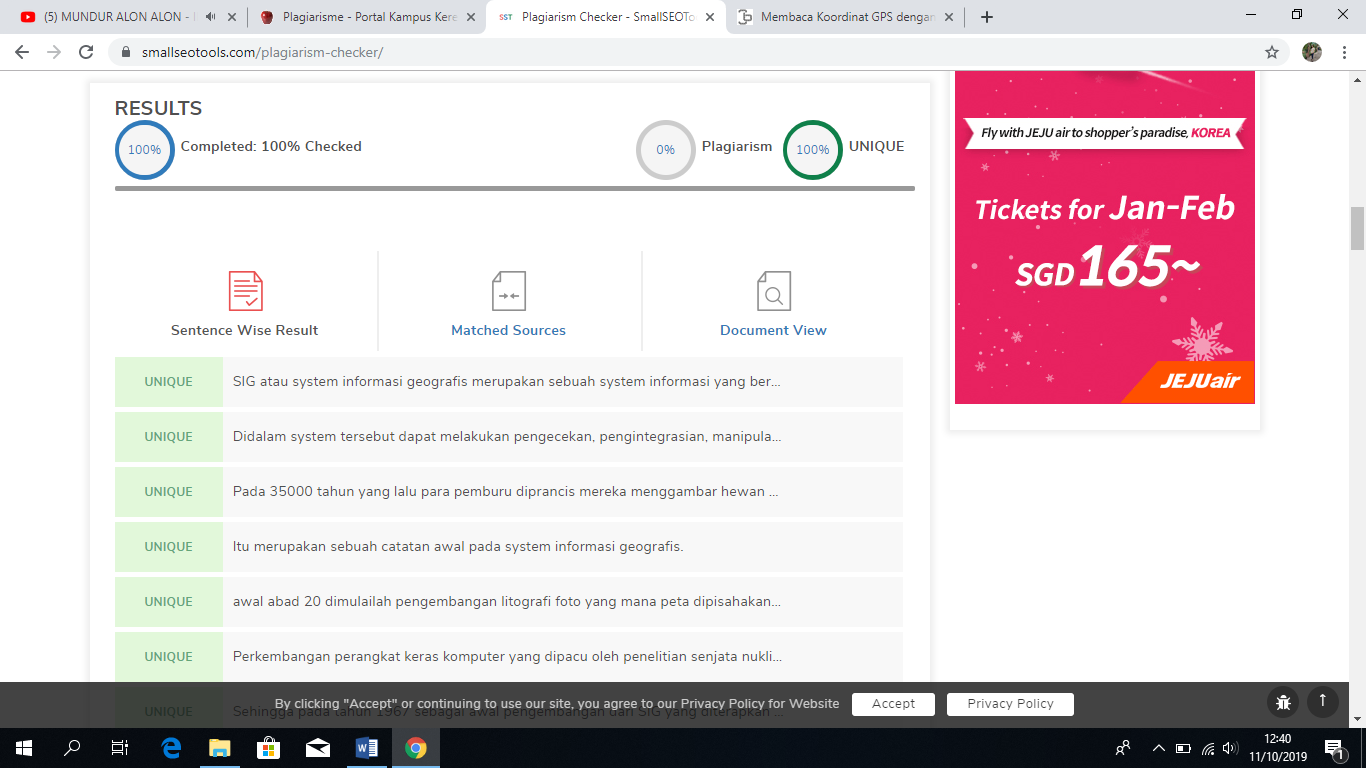
\includegraphics[width=4cm]{figures/1174012/gb.png}
	\centering
	\caption{Bukti}
\end{figure}
\section{DEZHA AIDIL MARTHA (1174025)}
\subsection{Pengertian}
Geografi adalah suatu ilmu yang mempelajari dan mendalami tentang lokasi suatu sistem peta, serta persamaan dan perbedaan variasi keruangan atas fenomena fisik, dan manusia di atas permukaan bumi. Geografi berasal dari Bahasa Yunani yaitu gêo "Bumi", dan graphein "Gambaran" atau "Menjelaskan". Para sarjana, praktisi, atau penulis di bidang Geografi disebut Geograf atau Geografer.Geografi juga merupakan nama judul buku bersejarah pada subjek ini, yang terkenal adalah Geographia tulisan Klaudios Ptolemaios pada abad-2.Geografi lebih dari sekadar kartografi, studi tentang peta. Geografi bukan hanya membahas apa, dan di mana di atas muka bumi, tapi juga mengapa sesuatu ada di situ, dan tidak di tempat lainnya, kadang bisa diartikan dengan "lokasi pada ruang." Geografi mempelajari hal ini, baik yang disebabkan oleh alam atau manusia. Juga mempelajari akibat yang disebabkan dari perbedaan yang terjadi itu.\hfill\break
Sistem informasi geografis (SIG) adalah sistem yang didesain untuk menangkap, menyimpan, mengolah, menganalisa, serta mempresentasikan data spasial.Dengan menghubungkan berbagai jenis data yang awalnya dianggap tidak berhubungan, SIG dapat membantu manusia dalam berbagai aspek pekerjaan. Proses menghubungkan ini umumnya dilakukan dalam konteks lokasi (spasial) dan waktu (temporal) yang sama.
\subsection{Sejarah}
Pada awalnya, peta hanya memiliki satu atau dua informasi saja didalamnya, sehingga jika seorang analis ingin mendapatkan informasi tambahan, dia harus melakukan overlay.Salah satu proses overlay pertama yang juga dianggap sebagai penerapan analisa spasial pertama secara sukses adalah oleh ilmuan / Geografer John Snow di London pada tahun 1854. Dia melakukan pemetaan terhadap lokasi orang-orang yang mengidap penyakit cholera dan menghubungkannya dengan peta penyediaan air minum London.\hfill\break
Pada awal abad ke-20, penggunaan teknik photozincography mulai meluas. Teknik ini memungkinkan peta terdiri dari beberapa layer yang nantinnya dapat diubah secara mandiri dari layer lainnya. Hal ini berguna untuk melakukan overlay dan analisa peta sesuai dengan layer yang dibutuhkan.Pada teknik ini, layer-layer yang ada dibuat dari film plastik atau lapisan kertas kalkir sehingga dapat digabungkan menjadi satu peta besar. Akan tetapi, teknik ini belum dapat dianggap sebagai SIG karena tidak terdapat database yang menghubungkan peta-peta tersebut.Pada tahun 1960, Canada mengembangkan sistem SIG pertamanya yang disebut CGIS atau Canada Geographic Information System. Sistem ini digunakan untuk menyimpan, mengolah, dan menganalisa informasi yang dimiliki oleh badan pertanahan Canada.
\subsection{Koordinat}
Koordinat didapatkan dari hasil perpotongan antara garis latitude (Y) / lintang dan garis longitude(X) / garis bujur sehingga bisa menunjukan suatu lokasi pada suatu daerah. \hfill\break 
Umumnya koordinat dibedakan menajadi koordinat Geografi dan Universal Transver Mercator(UTM). Pada koordinat geografi dibedakan menajadi 3 yaitu : \hfill\break
\begin{itemize}
	\item Degree, Decimal(DD, DDDD) contoh S 4.56734 E 102.67235
	\item Degree,Minute(DD MM,MMMM) contoh S 4 42,5423’ E 105 34,6445’
	\item Degree, Minute, Second(DD MM SS,SS) contoh : S 4 43’ 45,22 E 103 33’ 33,25
\end{itemize}
\hfill\break
\begin{figure}[H]
	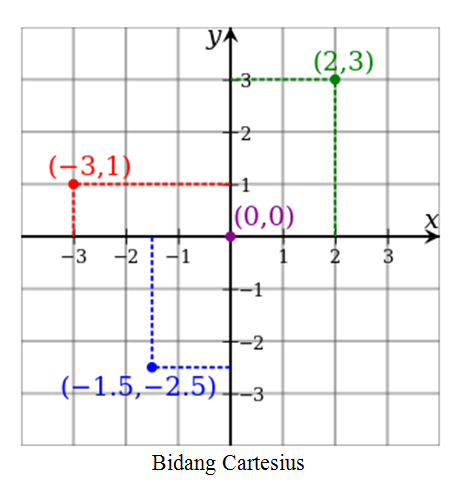
\includegraphics[width=4cm]{figures/1174025/1.png}
	\centering
	\caption{Contoh Koordinat}
\end{figure}
Pada system koordinat UTM biasanya terdapat pembagian waktu berdasarkan zonasinya. \hfill\break
\begin{figure}[H]
	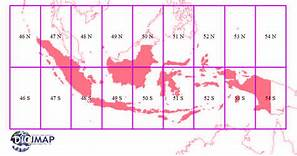
\includegraphics[width=4cm]{figures/1174025/2.jpg}
	\centering
	\caption{Contoh Koordinat UTM}
\end{figure}

\subsection{Data Geospasial}
Data geospasial merupakan pengambaran lokasi geografis,dimensi atau ukuran / karakteristik objek alam atau buatan manusia yang berada di bawah atau di atas permukaan bumi, data geospasial biasanya di singkat menjadi DG.
\hfill\break
Data Geospasial dibagi menjadi 3 yaitu :
\begin{itemize}
	\item Vektor
	Vektor merupakan salah jenis gambar yang dapat dibuat menggunakan aplikasi corel / adobe illustrator / aplikasi vektor lainnya. \hfill\break 
	Vektor itu sering digunakan untuk membuat gambar animasi dan vektor juga digunakan oleh goole maps.
	\item Roshen
	Roshen merupakan gambar yang di ambil dari satelit di luar angkasa, gambar ini biasanya bertipe jpg, dan pembaharuan data gambar ini berlangsung lama karena proses nya yang memakan waktu cukup banyak, jenis data ini digunakan oleh google earth.
	\item Roster
Data roster adalah data yang direpresentasikan dengan piksel dalam sebuah grafik. Data raster dihasilkan langsung oleh foto udara maupun foto satelit. Sehingga, secara umum, data roster lebih mudah dibuat dibandingkan dengan data vektor.
\end{itemize}

\subsection{Link}
\href{https://www.youtube.com/watch?v=Rw-D2J1h480}{Penjelasan GIT - Lalita Chandiany}
\subsection{Plagiarism}
\begin{figure}[H]
	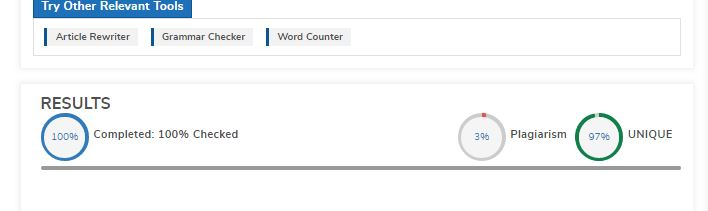
\includegraphics[width=4cm]{figures/1174025/plagiat.jpg}
	\centering
	\caption{Plagiat}
\end{figure}

\section{Dwi Septiani Tsaniyah{1174003}}

\subsection{Pengertian}
Istilah pada sistem informasi sistem geografis adalah untuk digunakan sebagai pendekatan sebuah sistem yang digunakan dalam sistem informasi geografis , dengan lingkungan yang komponen nya terpisah-pisah,sistem yang digunakan untuk mempermudah pemahaman yang terintegrasi. Pada saat ini teknologi komputer sangat banyak digunakan oleh banyak orang jadi hampir semua sistem informasi nya berdasarkan dengan pada komputer.
Kata informasi berasal dari sebuah pengolahan sejumlah data, di dalam sistem informasi geografis informasi mempunyai volume yang sangat besa. Pada setiap objek geografi memiliki settingan data yang berbeda beda , data tersendiri karena tidak sepenuhnya data yang ada terdapat di dalam peta. Jadi semua data harus diasosiasikan terlebih dahulu untuk menjadi peta yang inteligent, pada data tersebut mampu menampilakn atau memberikan sebuah informasi dengan hanya mengklik mouse pada suatu objek.
Pada istilah geografi ini digunakan karena sistem informasi geografis yang dibangun secara berdasarkan pada geografi. Pada objek ini lebih mengarah pada sfesifikasi lokasi. Objek ini bisa berupa fisik,budaya ataupun ekonomi alamiah. Pada objek ini penampakan nya bisa dilihat didalam sebuah peta yang dimana untuk memberikan sebuah gambaran yang refresentatif dari suatu objek yang sesuai dengan kenyataan di bumi. Pada saat ini teknologi telah membantu proses pemetaan.

\subsection{Sejarah}
Sejarah geografi dimulai sejak manusia mulai berinteraksi dengan lingkunganya, hal ini juga merupakan awal mula dari berkembangnya ilmu pengetahuan tentang geografi.
Pada awal dikenalnya sistem informasi geografis bahwa tidak lepas dari adanya kemajuan didalam bidang teknologi. Pada awal tahun 1960 perkembangan sistem informasi geografis dalam ilmu komputer semakin pesat dan siap dingunakan pada bidang milliter. Pada taun 1700 teknik yang digunakan pada survei modern untuk pemetaan topografis digunakan atau diterapkan , hal ini juga termasuk pada versi awal pemetaan tematis.

\subsection{Koordinat}
Koordinat adalah suatu titik yang didapatkan dari hasil perpotongan dari garis latitude (lintang) dengan garis bujur (longitude) sehingga akan menunjukan lokasi pada suatu daerah. Umumnya koordinat dibedakan menjadi koordinat Geographic dan Universal Transver Mercator (UTM). Pada Koordinat Geogprahic dibedakan menjadi tiga berdasarkan satuannya yaitu :
Koordinat adalah suatu titik yang didapatkan dari hasil pemotongan sebuah garis lintang dengan garis bujur sehingga akan menunjukan sebuah lokasi pada suatu daerah. Pada Bujur/Longitude (X) merupakan garis yang perpindahannya secara vertical dan pada Lintang/Lattitude (Y) merupakan garis yang mempunyai perpindahan secara horizontal, pada (Gambar 1) menjelaskan perpotongan antara garis bujur dan garis lintang akan membentuk suatu titik pertemuan yang biasa disebut dengan titik koordinat.
dibedakan menajadi 3 yaitu : 
\begin{itemize}
	\item Degree, Decimal(DD, DDDD) contoh S 4.56734 E 102.67235
	\item Degree,Minute(DD MM,MMMM) contoh S 4 42,5423’ E 105 34,6445’
	\item Degree, Minute, Second(DD MM SS,SS) contoh : S 4 43’ 45,22 E 103 33’ 33,25
\end{itemize}
\hfill\break
\begin{figure}[H]
	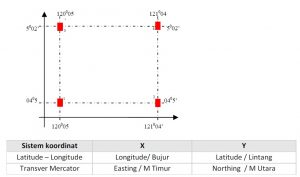
\includegraphics[width=4cm]{figures/1174003/koordinat.jpg}
	\centering
	\caption{Contoh Koordinat}
\end{figure}

\subsection{Data Geospasial}
Geospital data tentang suatu aspek fisik dari sebuah objek yang geografis , misalnya seperti bentuk alam tentu saja sungai,danau,pantai dan bentuk alam lainnya. Secara umun terdapat 2 fitur untuk menampilkan yaitu termasuk ke dalam geografis dan sistem informasi geospasial. Dalam struktur data yang demikian didalam nya ada unsur resolusi sebagai ukuran dari dimensi fitur geografis
Data Geospasial dibagi menjadi 2 yaitu :
\begin{itemize}
	\item Vektor
	Vektor merupakan salah jenis gambar yang dapat dibuat menggunakan aplikasi corel / adobe illustrator / aplikasi vektor lainnya.
	Vektor itu sering digunakan untuk membuat gambar animasi dan vektor juga digunakan oleh goole maps.
	\item Roshen
	Roshen merupakan gambar yang di ambil dari satelit di luar angkasa, gambar ini biasanya bertipe jpg, dan pembaharuan data gambar ini berlangsung lama karena proses nya yang memakan waktu cukup banyak, jenis data ini digunakan oleh google earth.
\end{itemize}
\subsection{Link}
\begin{itemize}
	\item \href{https://youtu.be/CXKVVDaUo30}{Materi GIS}
\end{itemize}
\subsection{Plagiarism}
\begin{figure}[H]
	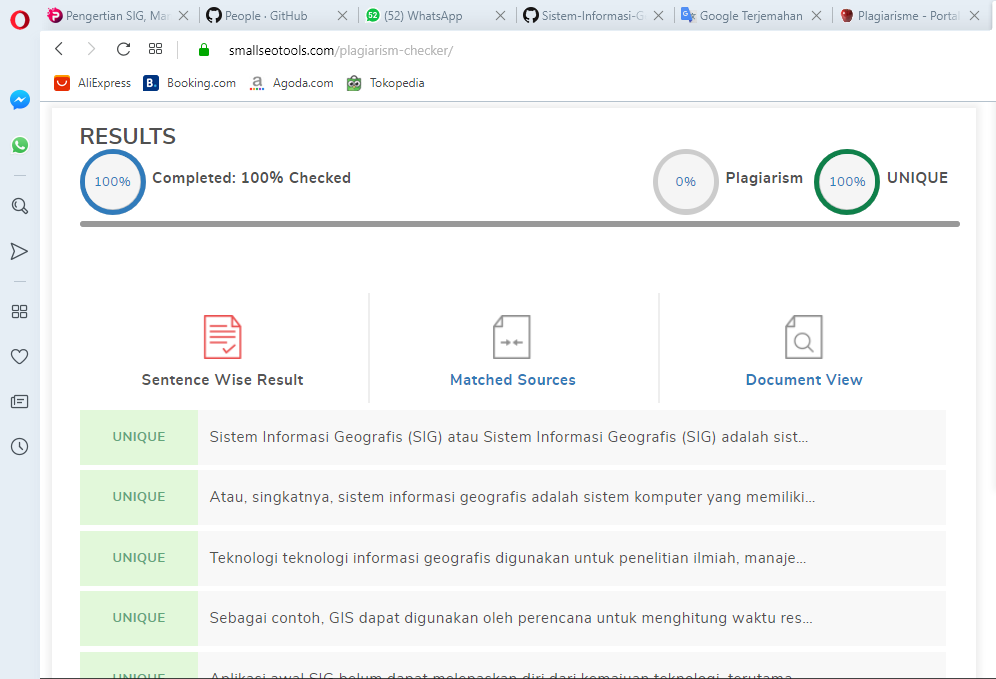
\includegraphics[width=4cm]{figures/1174003/1174003_plagiarisme.png}
	\centering
	\caption{Bukti Tidak Melakukan Plagiat}
\end{figure}
\section{Dwi Yulianingsih(1174009)}
\subsection{Pengertian}
Sistem informasi geografis merupakan sebuah aplikasi /system pengolah data spasial yang memanfaatkan system komputerisasi dengan menggabungkan data grafis dan data atribut objek memanfaatkan peta dasar digital dengan referensi yang digunakan yaitu bumi. SIG pada dasarnya akan memunculkan dan memberi data-data yang diinginkan oleh user dimana dulunya manual yang diperbaharui menjadi data digital terkomputerisasi. System informasi geografis digunakan untuk mengumpulkan, mengubah, mengevaluasi, serta mengawasi seluruh data bumi yang dibutuhkan oleh user, dulunya data disimpan secara manual yang memungkinkan data bisa hilang/ rusak maka diperbaharui agar lebih mudah dan aman.

\subsection{Sejarah}
Sejarah dari SIG kurang lebih adalah sebagai berikut :
\begin{itemize}
\item Pada tahun 1960 ilmu computer mulai berkembang pesat dan siap digunakan untuk berbagai bidang. Ahli meteorology, geologi, dan 	geofisika mulai mengikuti perkembangan zaman dan memanfaatkannya  untuk membuat peta.
\item  Pada 1963 muncul Canadian geographic information system (CGIS) di Kanada dan menjadi system informasi geografis pertama di dunia. Dua tahun kemudian Amerika mulai mengikuti jejak Kanada dengan MIDAS-nya untuk memproses data SDA yang ada disana. 
\item Pada 1967 perkembangan awal SIG diterapkan di Ottawa, Ontario oleh departemen energi pertambangan dan sumber daya (ini merupakan perkembangan dari Canadian geographic information system yang digunakan untuk inventarisasi tanah Kanada (CLI) untuk mengetahui kemampuan memetakan informasi geologi disana).  
\item CGIS memiliki aplikasi pemetaan yang berkemampuan timpang susun atau overlay, perhitungan, pemindaian, system koordinat, dan topologi yang menyimpan atribut dan lokasional dalam berkas terpisah. CGIS ini bertahan sampai tahun 1970-an dan disempurnakan agar bisa bersaing dengan aplikasi pemetaan lain yang di keluarkan oleh vendor-vendor seperti Intergraph. 
\item Perkembangan yang terus menerus terjadi memacu pemtumbuhan SIG dapat dijalankan di workstation unix dan computer pribadi dengan standar platform yang lebih sedikit dan user yang mulai mengekplor data SIG lewat internet hingga bisa menjadi seperti sekarang.
\end{itemize}

\subsection{Koordinat}
Koordinat merupakan titik-titik yang didapat dari hasil pertemuan garis latitude dan longitude atau lintang dan bujur sehingga dapat menunjukan lokasi sebuah daerah/tempat. Pada umumnya koordinat dibedakan menjadi dua yaitu koordinat geograpik dan UTM. Di koordinat geograpik ada 3 satuan yaitu :
\begin{itemize}
\item Degree, Decimal (DD,DDDD) Contoh : S 3.56734 E 104.67235
\item Degree, Minute (DD MM,MMMM) Contoh : S 3' 43,5423' E 104 33,6445'
\item Degree, Minute, Second (DD MM SS,SS) Contoh : S 3' 43' 45,22'' E104 33' 33,25''
\end{itemize}

\begin{figure}[H]
	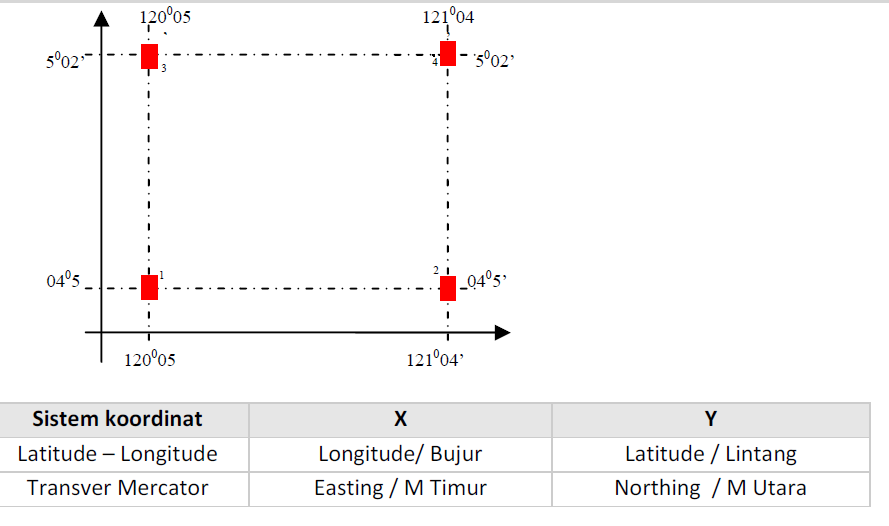
\includegraphics[width=5cm]{figures/1174009/t1.png}
	\centering
	\caption{geographic}
\end{figure}

Pada system UTM terbagi menjadi beberapa  waktu tergantung pada zonasinya, diindonesia waktu dibagi menjadi 16 zonasi seperti pada gambar di bawah :
\begin{figure}[H]
	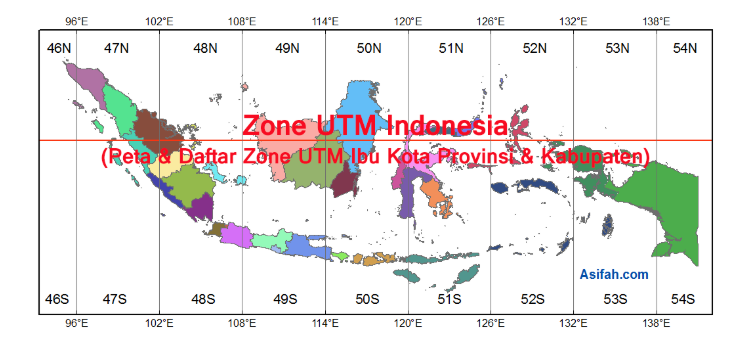
\includegraphics[width=5cm]{figures/1174009/t2.png}
	\centering
	\caption{UTM}
\end{figure}

\subsection{Data Geospasial}
Data geospasial adalah data yang memuat informasi spesifik mengenai fisik dan administrative dari sebuah objek. Aspek yang termasuk fisik disini seperti bentuk alam di permukaan (bumi) yang mengandung fenomena seperti jalan, rel kereta api, jembatan, bangunan dan sebagainya selain itu juga seperti aliran sungai, dataran tinggi, pantai, danau dan sebagainya. Termasuk juga aspek administrative seperti batas negara, pembagian wilayah, zona, postal code, batas tanah dan lainnya. Sebuah objek biasanya dikaitkan dengan atribut dari objeknya dan informasinya dapat di letakkan terpisah dengan pangkalan data induknya. Ada dua metode dalam data geospasial ini ada data vector dan data raster. Data vector terdiri dari gambaran titik geografis mau berupa titik, garis maupun polygon. Sementara data raster terdiri dari pixels yang digunakan untuk mrnggambarkan data yang berhubungan. 
\begin{figure}[H]
	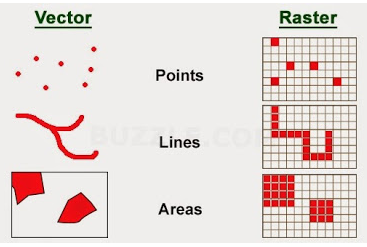
\includegraphics[width=5cm]{figures/1174009/t3.png}
	\centering
	\caption{geopasial}
\end{figure}

\subsection{Link Video}
\href{https://youtu.be/MXutHP_22_M}{Yuk lihat videonya}

\subsection{Plagiarism}
\begin{figure}[H]
	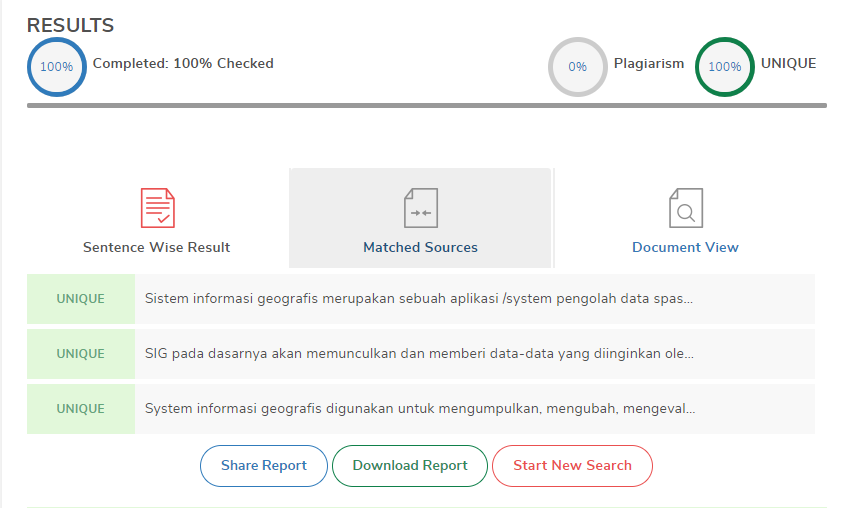
\includegraphics[width=5cm]{figures/1174009/plagiat1.png}
	\centering
	\caption{Bukti Tidak Plagiat}
\end{figure}

\begin{figure}[H]
	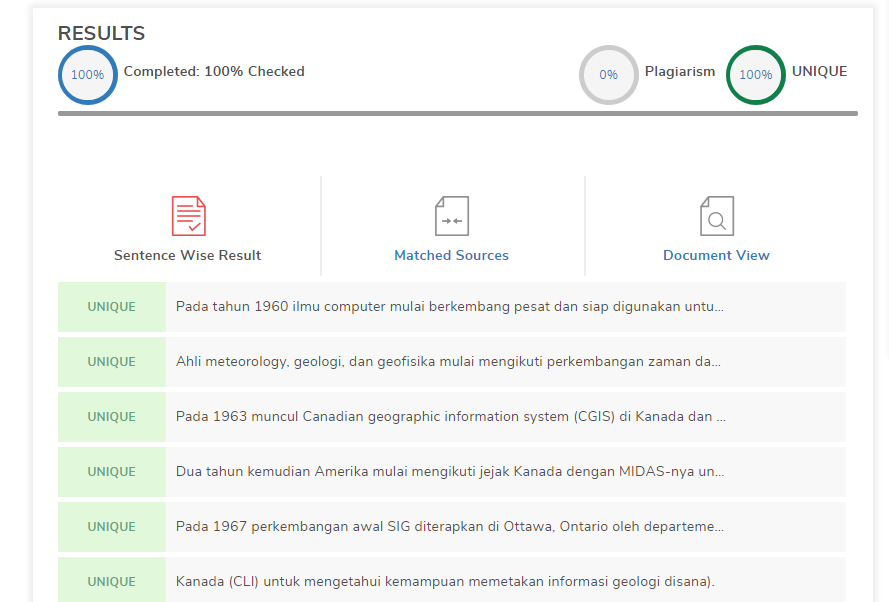
\includegraphics[width=5cm]{figures/1174009/plagiat2.png}
	\centering
	\caption{Bukti Tidak Plagiat}
\end{figure}

\begin{figure}[H]
	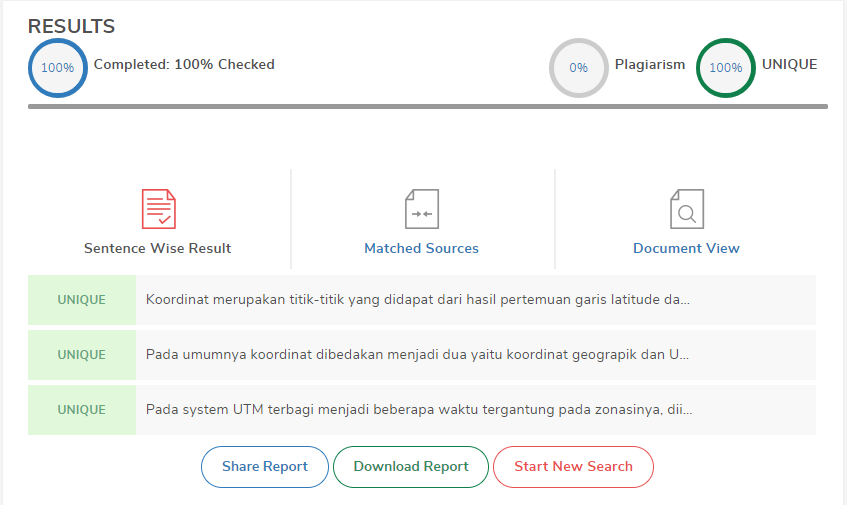
\includegraphics[width=5cm]{figures/1174009/plagiat3.png}
	\centering
	\caption{Bukti Tidak Plagiat}
\end{figure}

\begin{figure}[H]
	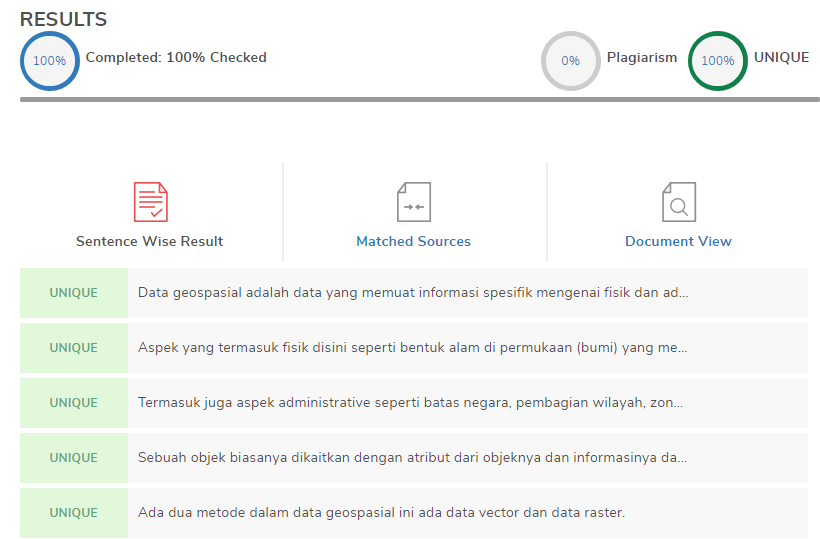
\includegraphics[width=5cm]{figures/1174009/plagiat4.png}
	\centering
	\caption{Bukti Tidak Plagiat}
\end{figure}

\section{Evietania Charis Sujadi (1174051)}
\subsection{Pengertian}
adalah suatu sistem informasi yang berbasis komputer, dirancang untuk bekerja dengan menggunakan data yang memiliki informasi spasial . Sistem ini mengcapture, mengecek, mengintegrasikan, memanipulasi, menganalisa, dan menampilkan data yang secara spasial mereferensikan kepada kondisi bumi. \hfill\break
Aktifitas yang terjadi di bumi merupakan bagian dari ilmu Geografi.\hfill\break
\subsection{Sejarah}
pada 35000 tahun yang lalu, pada dinding gua Lascaux, Perancis, para pemburu Cro-Magnon menggambar hewan mangsa mereka, juga garis yang dipercaya sebagai rute migrasi hewan-hewan tersebut. pada catatan awal ini sejalan dengan dua elemen struktur pada sistem informasi gegrafis modern sekarang ini, arsip grafis yang terhubung ke database atribut.\hfill\break
Pada tahun 1700an sebuah teknik survey modern untuk pemetaan topografis diterapkan, termasuk versi awal pemetaan tematis, misalnya untuk keilmuan atau data sensus.\hfill\break
pada awal abad ke 20 memperlihatkan pengembangan “litografi foto” dimana peta dipisahkan menjadi beberapa lapisan . Perkembangan perangkat keras komputer yang dipacu oleh penelitian senjata nuklir membawa aplikasi pemetaan menjadi multifungsi pada awal tahun 1960an.\hfill\break
Pada tahub 1967 merupakan awal pengembangan SIG yang bisa diterapkan di Ottawa, Ontario oleh Departemen Energi, Pertambangan dan Sumber Daya. dikembangkan oleh roger dimana, kemudian disebut CGIS (Canadian GIS – SIG Kanada), digunakan untuk menyimpan, menganalisis dan mengolah data yang dikumpulkan untuk Inventarisasi Tanah Kanada (CLI) sebuah inisiatif untuk mengetahui kemampuan lahan di wilayah pedesaan Kanada dengan memetakaan berbagai informasi pada tanah, pertanian, pariwisata, alam bebas, unggas dan penggunaan tanah pada skala 1:250000.\hfill\break
CGIS bertahan sampai tahun 1970-an dan memakan waktu lama untuk penyempurnaan setelah pengembangan, dan tidak bisa bersaing denga aplikasi pemetaan komersil yang dikeluarkan beberapa vendor seperti Intergraph. Perkembangan perangkat keras mikro komputer memacu vendor lain seperti ESRI dan CARIS berhasil membuat banyak fitur SIG, menggabung pendekatan generasi pertama pada pemisahan informasi spasial dan atributnya, dengan pendekatan generasi kedua pada organisasi data atribut menjadi struktur database. Perkembangan industri pada tahun 1980 dan 1990 memacu sebuah pertumbuhan SIG pada workstation UNIX dan komputer pribadi. Pada akhir abad ke 20, pertumbuhan yang cepat di berbagai sistem dikonsolidasikan dan distandarisasikan menjadi platform lebih sedikit, dan para pengguna mulai mengekspor menampilkan data SIG lewat internet, yang membutuhkan standar pada format data dan transfer
\subsection{Koordinat}
Koordinat didapatkan dari hasil perpotongan antara garis latitude (Y) / lintang dan garis longitude(X) / garis bujur sehingga bisa menunjukan suatu lokasi pada suatu daerah.
\subsection{Data Geospasial}
Data yang aspek fisiknya dan administratif dari sebuah objek geografis. Aspek fisik di sini mencakup pula bentuk anthropogenic dan bentuk alam baik yang terdapat di permukaan maupun di bawah permukaan bumi. 
\subsection{Link}
\href{https://youtu.be/eby2SXgrvbU}{Pencet Aku}
\subsection{Plagiarism}
\begin{figure}[H]
	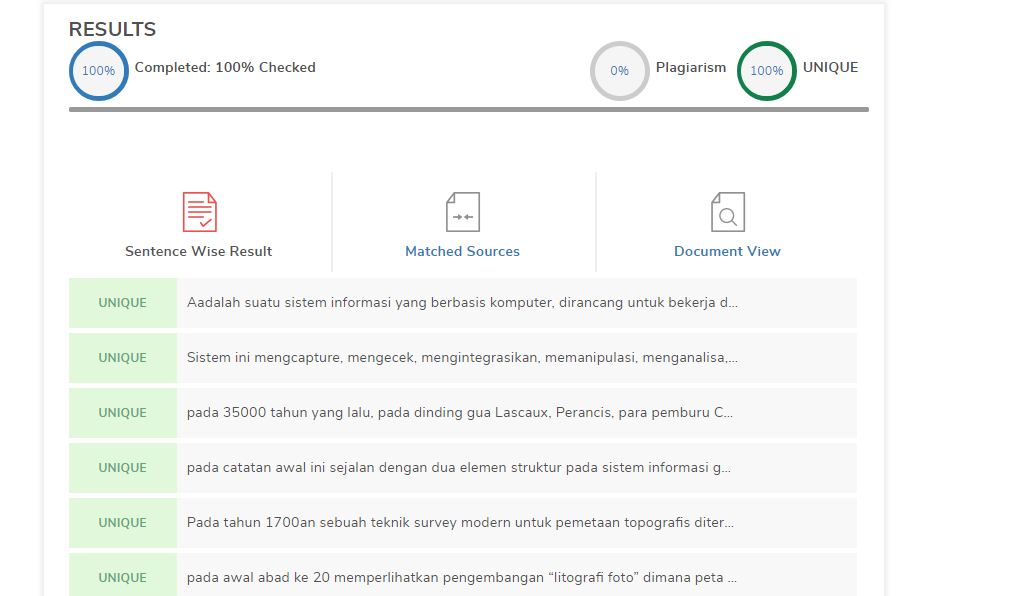
\includegraphics[width=4cm]{figures/1174051/1/1.png}
	\centering
	\caption{Bukti Tidak Melakukan Plagiat}
\end{figure}

\subsubsection{List}
\begin{enumerate}
	\item Satu
	\item Dua
\end{enumerate}

\begin{itemize}
	\item Satu
	\item Dua
\end{itemize}

\href{link kamu}{alias}
contoh link
\href{https://www.google.com/}{klik me}
\section{Felix Setiawan Lase (1174026)}
\subsection{Pengertian}
Pada dasarnya istilah sistem informasi geografis adalah kombinasi dari tiga elemen utama yaitu sistem, informasi, dan geografi.
Sistem adalah kumpulan benda, ide, dan hubungan mereka dalam mencapai tujuan bersama.\hfill\break
Sistem informasi adalah sistem antara manusia dan mesin yang terintegrasi untuk menyajikan informasi untuk mendukung fungsi operasi, manajemen, dan pengambilan keputusan dalam organisasi.\hfill\break
Penggunaan istilah informasi geografis menyiratkan informasi tentang tempat-tempat yang terletak di permukaan bumi. Pengetahuan tentang posisi di mana objek berada di permukaan bumi dan informasi tentang informasi dan posisi yang terkandung di permukaan bumi.
\subsection{Sejarah}
Pengenalan awal GIS tidak lepas dari kemajuan di bidang teknologi, khususnya komputer. Selama perang dunia kedua pemrosesan data mengalami kemajuan pesat terutama untuk memenuhi kebutuhan militer dalam memprediksi lintasan balistik. Pada awal 1960-an perkembangan ilmu komputer berkembang pesat dan siap digunakan untuk bidang lain di luar militer. Ahli meteorologi, geologi dan geofisika mulai menggunakan komputer dalam pembuatan peta.\hfill\break

Pada tahun 1963 di Kanada muncul CGIS (Sistem Informasi Geografis Kanada), dan kemudian menjadi GIS pertama di dunia. Dua tahun kemudian di Amerika Serikat mengoperasikan sistem serupa yang disebut MIDAS yang digunakan untuk memproses data sumber daya alam.
\subsection{Koordinat}
Koordinat adalah titik yang diperoleh dari perpotongan garis lintang (garis lintang) dengan garis bujur (garis bujur) sehingga akan menunjukkan lokasi di suatu daerah. Secara umum koordinat dibagi menjadi Koordinat Geografis dan Universal Transver Mercator (UTM)
\subsection{Data Geospasial}
\begin{enumerate}
	\item Data global positioning system (GPS). Data GPS dikumpulkan melalui sistem navigasi radio berbasis satelit dan darat. Smartphone yang mampu GPS dapat memberikan lokasi seseorang.
	\item Data penginderaan jauh. Penginderaan jauh melibatkan instrumen khusus yang menangkap data yang dapat dikonversi menjadi bentuk digital. 
\end{enumerate}\hfill\break

Foto udara dapat digunakan untuk mengenali beberapa objek di muka bumi. Dengan menganalisis bentuk, ukuran dan warna benda-benda ini, kita dapat mengamati keberadaan tanah basah atau kering, tanaman atau penyakit yang sehat, dan sawah irigasi atau tadah hujan. Tanah basah akan lebih gelap jika dibandingkan dengan tanah kering.

Data geospasial banyak berguna, baik untuk bisnis maupun untuk pemerintah.\hfill\break

Sebagai contoh, dengan data geospasial kita dapat melihat jalan mana yang padat atau bahkan padat. Dengan mengetahui situasi ini, pihak berwenang seperti polisi dapat melakukan penanganan seperti mengalihkan arus ke rute alternatif atau menerapkan jalan satu arah.

\subsection{Link}
\begin{itemize}
	\item \href{https://youtu.be/GOjKvnfiYC8}{Lihat Disini}
\end{itemize}
\subsection{Plagiarism}
\begin{figure}[H]
	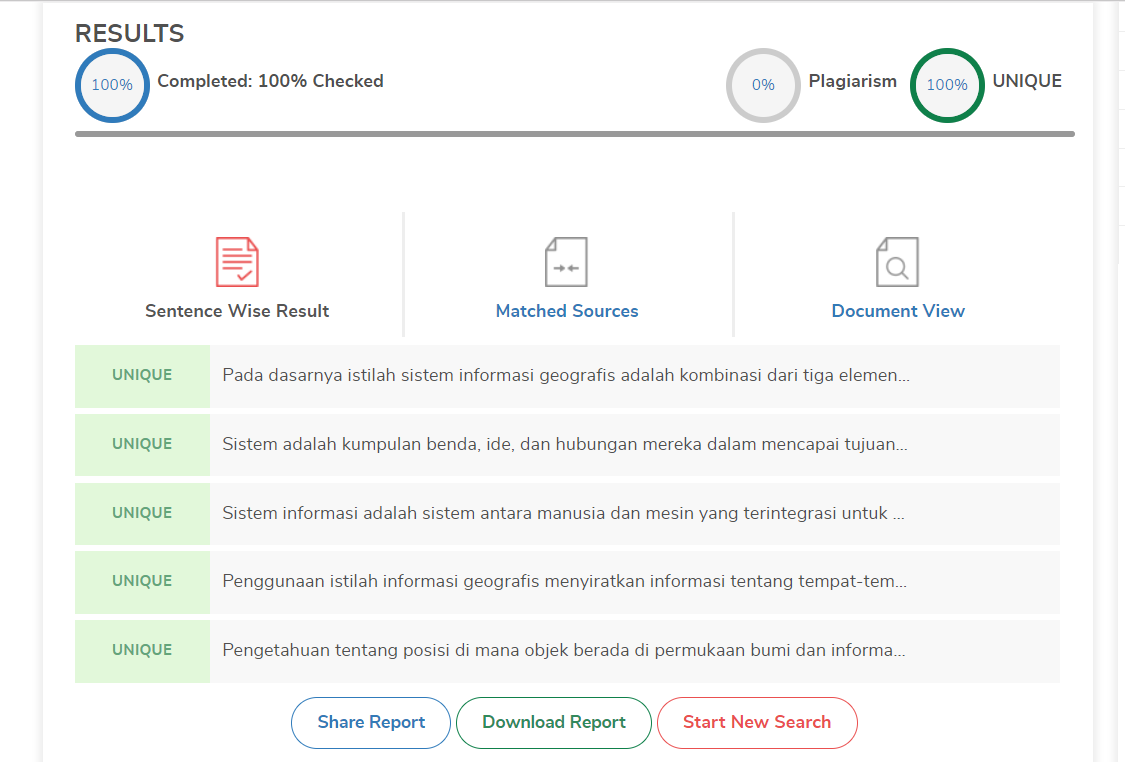
\includegraphics[width=4cm]{figures/1174026/1/1.png}
	\centering
	\caption{Bukti Tidak Melakukan Plagiat}
\end{figure}
\begin{figure}[H]
	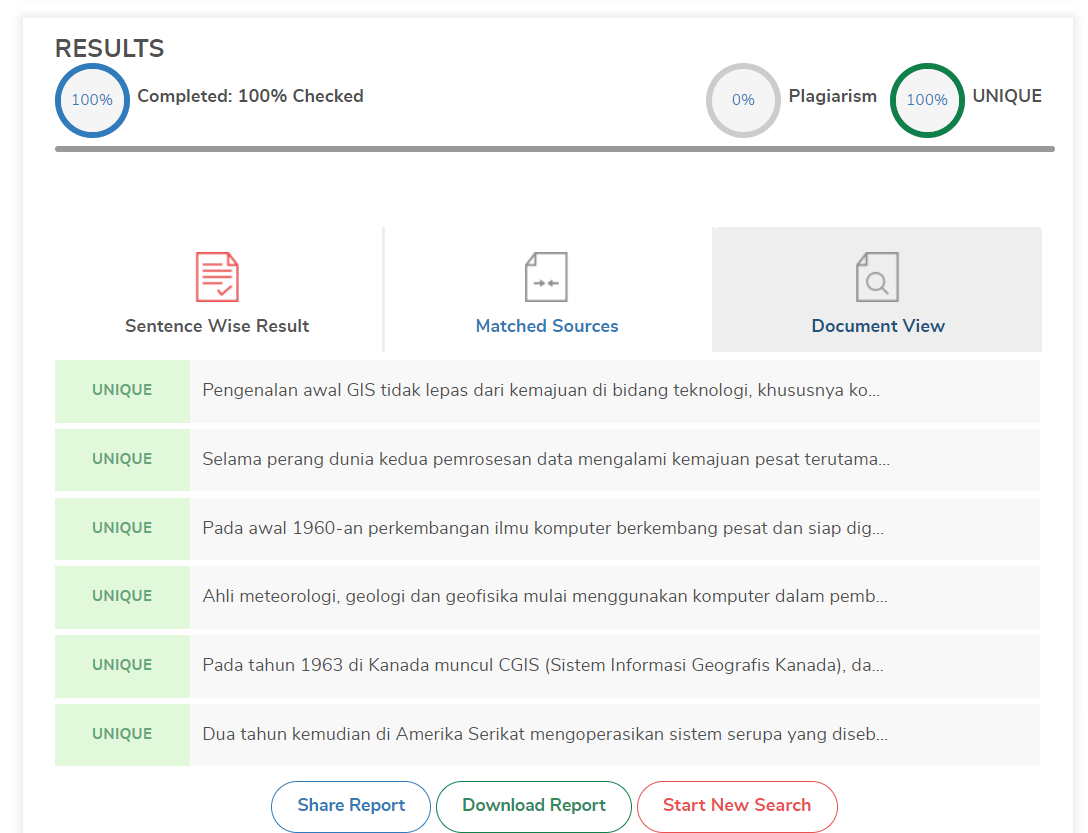
\includegraphics[width=4cm]{figures/1174026/1/2.png}
	\centering
	\caption{Bukti Tidak Melakukan Plagiat}
\end{figure}
\begin{figure}[H]
	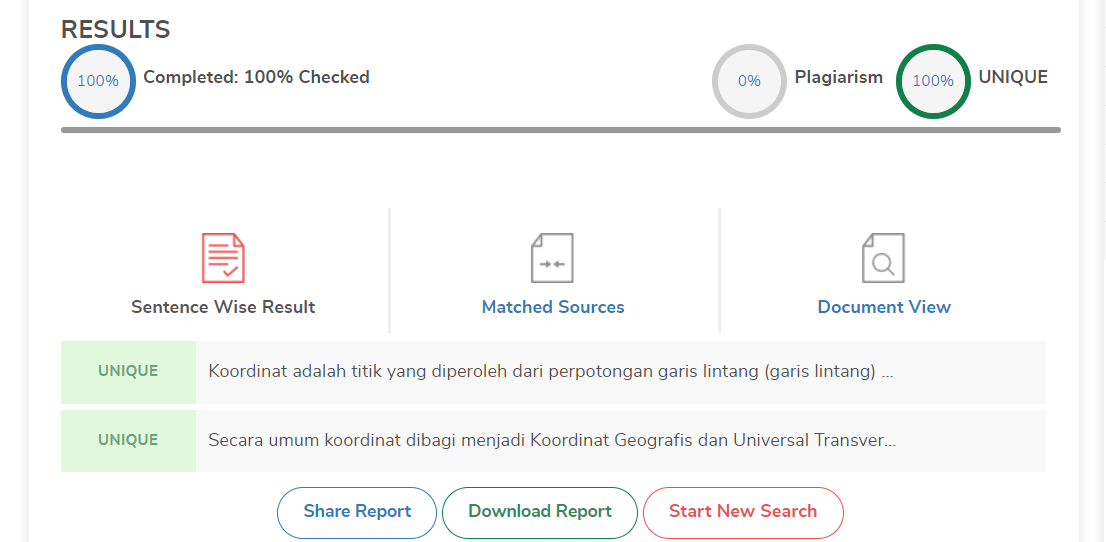
\includegraphics[width=4cm]{figures/1174026/1/3.png}
	\centering
	\caption{Bukti Tidak Melakukan Plagiat}
\end{figure}
\begin{figure}[H]
	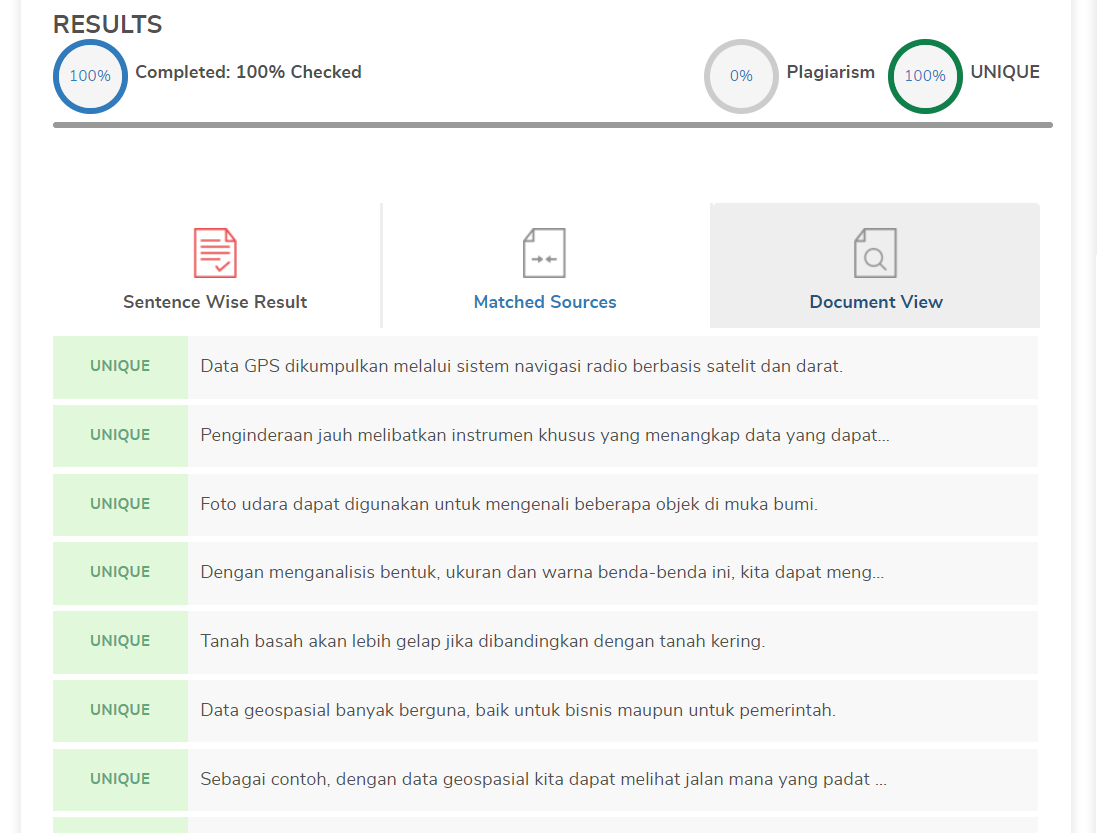
\includegraphics[width=4cm]{figures/1174026/1/4.png}
	\centering
	\caption{Bukti Tidak Melakukan Plagiat}
\end{figure}



\section{NAMA (NPM)}
\subsection{Pengertian}
\subsection{Sejarah}
\subsection{Koordinat}
\subsection{Data Geospasial}
\subsection{Link}
\subsection{Plagiarism}

\subsection{Cara Penggunaan}
\subsubsection{Gambar}

\hfill\break

Contoh Gambar
\begin{figure}[H]
	
\includegraphics[width=4cm]{figures/himatif.png}
	\centering
	\caption{Contoh gambar.}
\end{figure}

\subsubsection{List}
\begin{enumerate}
	\item Satu
	\item Dua
\end{enumerate}

\begin{itemize}
	\item Satu
	\item Dua
\end{itemize}

\href{link kamu}{alias}
contoh link
\href{https://www.google.com/}{klik me}
\section{Harun Ar - Rasyid(1174027)}
\subsection{Pengertian}
Geografi adalah ilmu pengetahuan yang mengambarkan segala sesuatu yang ada di permukaan bumi. \hfill\break
Geografi juga selain mempelajari bagian permukaan bumi, tapi juga mempelajari seluruh bagian bumi mulai darti struktur bumi,jenis batuan yang menyusun bumi serta atmosfer yang melindungi bumi. \hfill\break
Segala aktifitas yang terjadi di bumi merupakan bagian dari ilmu Geografi.\hfill\break
\subsection{Sejarah}
Sejarah geografi dimulai sejak manusia mulai berinteraksi dengan lingkunganya, hal ini juga merupakan awal mula dari berkembangnya ilmu pengetahuan tentang geografi.\hfill\break
Pada awalnya geografi hanya membahas atau mendekripsikan gambaran umum tentang fakta-fakta yang menjelaskan keadaan di muka bumi. Pada abad ke-18 yaitu masa geografi klasik, ilmu geografi hanya sebatas menjelaskan dan mengumpulkan informasi tentang lingkungan geografi saja, misalnya: keadaan politik, industri, iklim terutama di kota-kota besar.\hfill\break
Sejarah geografi terus berjalan dan berkembang. Tepatnya, diabad ke-19 geografi mengalami perkembangan dari segi keilmuannya. Dari yang semula hanya mendeskripsikan saja kemudian berkembang menjadi lebih spesifik yaitu dengan menjelaskan lingkungan geografi secara sistematis.\hfill\break
Pada pertengahan abad ke-19, keilmuan dalam geografi sudah membahas sampai ketingkat membandingkan keadaan, data geografis dan karakteristik antara wilayah yang satu dengan wilayah yang lain di muka bumi. Hal ini kita kenal sebagai “Comparative Geography”.\hfill\break
Perkembangan keilmuwan geografi semakin pesat pasca terjadinya perang dunia ke-II. Yang semula dikembangkan oleh imuwan Amerika dan Inggris yang dikenal sebagai “Comparative Geography” kemudian berkembang menjadi “Global Geography” dimana objek kajiannya semakin luas yaitu meliputi seluruh dunia. Era inilah yang dinamakan sebagai “era geografi modern”.\hfill\break
Dari pembahasan di atas, kita sudah mengetahui kapan sejarah geografi itu dimulai yaitu sejak adanya interaksi antara manusia dengan lingkungannya. Bila seperti itu, maka hakekatnya sejak Nabi Adam as turun ke bumi sebetulnya geografi sudah ada.\hfill\break
Akan tetapi penggalian geografi secara keilmuan sendiri baru dilakukan pertama kali oleh orang-orang Yunani. Dimana pada perkembangan awalnya dilatarbelakangi oleh suatu upaya masyarakat Yunani untuk melepaskan diri dari alam pikiran dan kepercayaan. Dimana kepercayaan tersebut meyakini bahwa dewa-dewa ikut turut campur dalam segala bentuk kejadian di bumi.\hfill\break
Istilah geografi sebenarnya baru digunakan pada tahun 1972 sedangkan sebelumnya lebih menggunakan istilah “ilmu bumi”. Istilah ini pertama kali diperkenalkan oleh seorang ahli filsafat dan astronomi yang bernama Eratosthenes pada 276 194 sebelum masehi.Kemudian, Claudius Ptoleumaeus melakukan peletakan dasar-dasar keilmuan geografi.\hfill\break
Sejarah perkembangan geografi terus berlanjut. Immanuel Kant mengembangkan geografi modern kemudian Karl Ritter juga mengembangkan geografi sosial.\hfill\break
Selain itu ada tokoh-tokoh lain yang ikut andil dalam mengembangkan geografi yaitu Alexander von Humbolt sebagai peletak dasar geografi fisika modern dan sebagainya.\hfill\break
\subsection{Koordinat}
Koordinat didapatkan dari hasil perpotongan antara garis latitude (Y) / lintang dan garis longitude(X) / garis bujur sehingga bisa menunjukan suatu lokasi pada suatu daerah. \hfill\break 
Umumnya koordinat dibedakan menajadi koordinat Geografi dan Universal Transver Mercator(UTM). Pada koordinat geografi dibedakan menajadi 3 yaitu : \hfill\break
\begin{itemize}
	\item Degree, Decimal(DD, DDDD) contoh S 4.56734 E 102.67235
	\item Degree,Minute(DD MM,MMMM) contoh S 4 42,5423’ E 105 34,6445’
	\item Degree, Minute, Second(DD MM SS,SS) contoh : S 4 43’ 45,22 E 103 33’ 33,25
\end{itemize}
\hfill\break
\begin{figure}[H]
	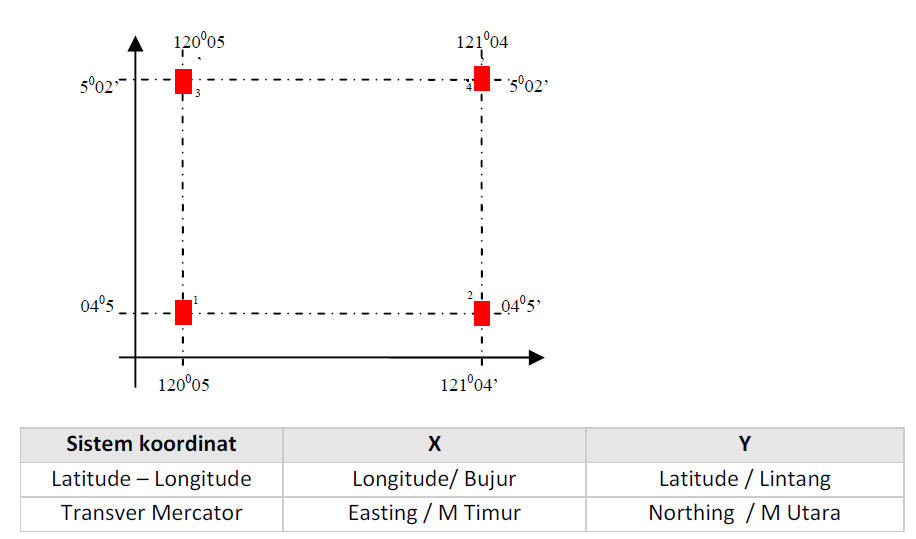
\includegraphics[width=4cm]{figures/1174027/1_1174027_koordinat.jpg}
	\centering
	\caption{Contoh Koordinat}
\end{figure}
Pada system koordinat UTM biasanya terdapat pembagian waktu berdasarkan zonasinya. \hfill\break
\begin{figure}[H]
	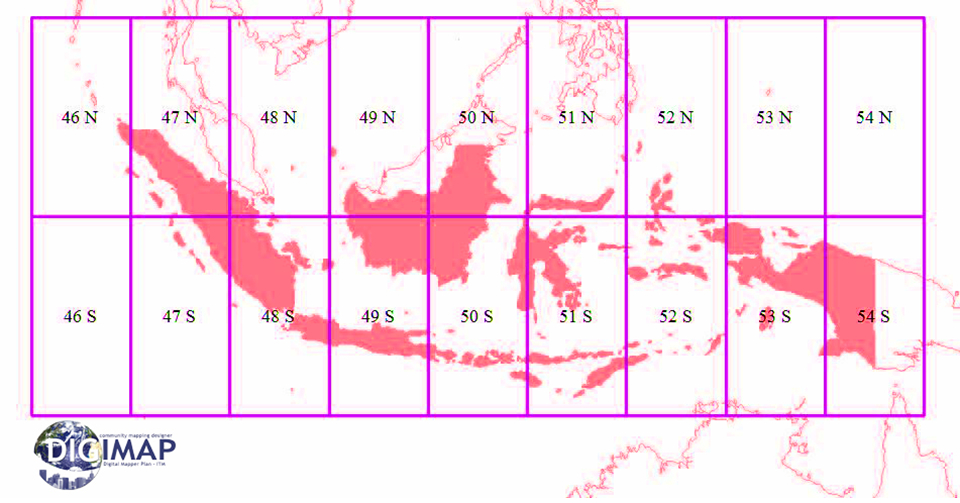
\includegraphics[width=4cm]{figures/1174027/1_1174027_UTM.jpg}
	\centering
	\caption{Contoh Koordinat UTM}
\end{figure}

\subsection{Data Geospasial}
Data geospasial merupakan pengambaran lokasi geografis,dimensi atau ukuran / karakteristik objek alam atau buatan manusia yang berada di bawah atau di atas permukaan bumi, data geospasial biasanya di singkat menjadi DG.
\hfill\break
Data Geospasial dibagi menjadi 2 yaitu :
\begin{itemize}
	\item Vektor
	Vektor merupakan salah jenis gambar yang dapat dibuat menggunakan aplikasi corel / adobe illustrator / aplikasi vektor lainnya. \hfill\break 
	Vektor itu sering digunakan untuk membuat gambar animasi dan vektor juga digunakan oleh goole maps.
	\item Roshen
	Roshen merupakan gambar yang di ambil dari satelit di luar angkasa, gambar ini biasanya bertipe jpg, dan pembaharuan data gambar ini berlangsung lama karena proses nya yang memakan waktu cukup banyak, jenis data ini digunakan oleh google earth.
\end{itemize}
\subsection{Link}
\begin{itemize}
	\item \href{https://youtu.be/mhk9PhmNLvk}{Pengertian GIS}
	\item \href{https://youtu.be/7K0x-oQncy4}{Sejarah GIS}
	\item \href{https://youtu.be/QE8uvqNqbo4}{Koordinat}
	\item \href{https://youtu.be/CXYenLiAS8U}{Data Geospasial}
\end{itemize}
\subsection{Plagiarism}
\begin{figure}[H]
	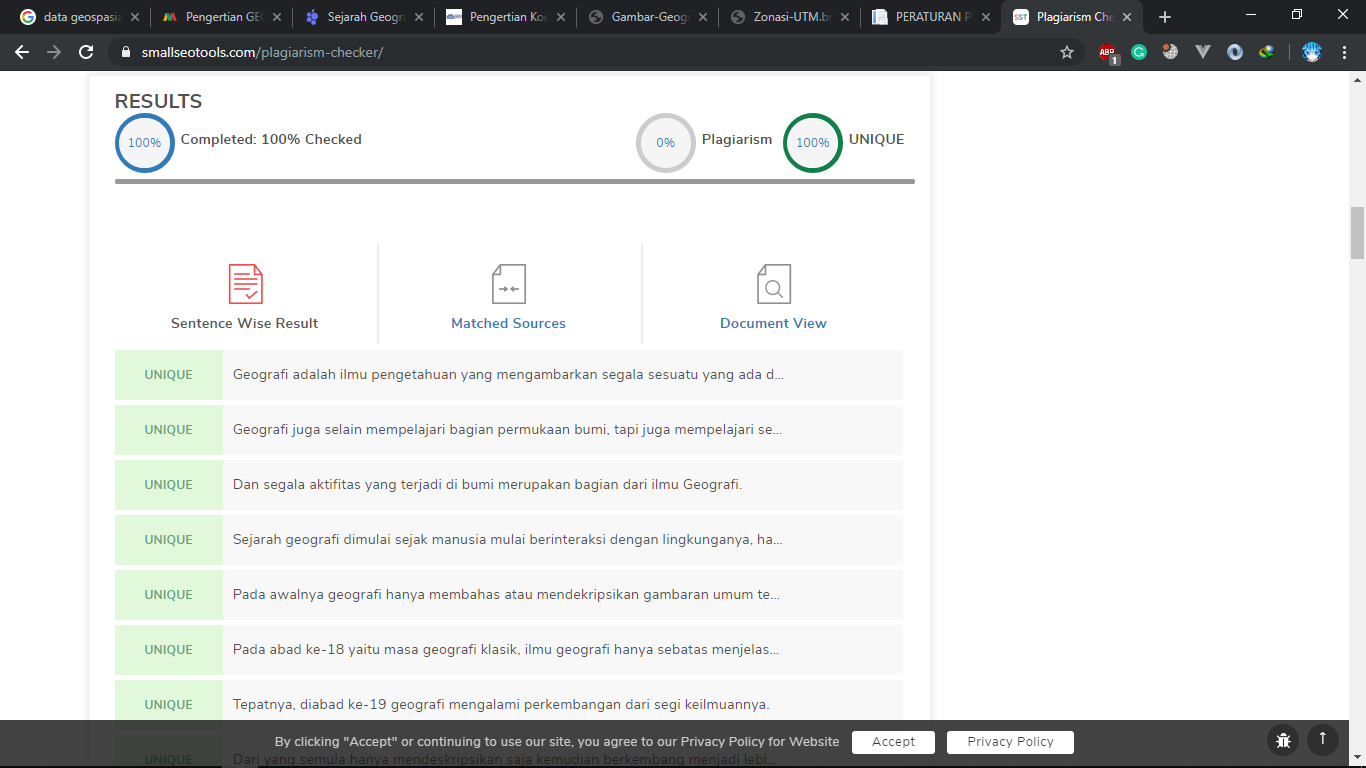
\includegraphics[width=4cm]{figures/1174027/1_1174027_placek.png}
	\centering
	\caption{Bukti Tidak Melakukan Plagiat}
\end{figure}
\section{Kadek Diva Krishna Murti (1174006)}
\subsection{Pengertian}
\begin{figure}[H]
	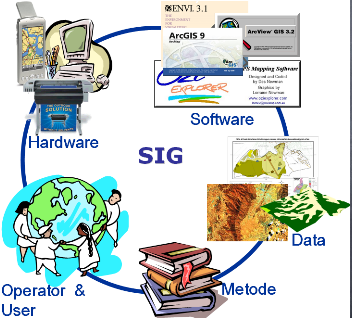
\includegraphics[width=4cm]{figures/1174006/1174006sig1.png}
	\centering
	\caption{Sistem Informasi Geografis.}
\end{figure}
Sistem Informasi Geografis merupakan sebuah runtutan kegiatan yang dilakukan untuk mendapatkan sebuah gambaran mengenai keadaaan ruang muka bumi atau informasi mengenai ruang muka bumi yang dibutuhkan untuk menjawab atau menyelesaikan suatu permasalahan yang ada pada ruang muka bumi yang bersangkutan. Runtutan kegiatan tersebut seperti pengumpulan, penataan, pengolahan, penganalisisan dan penyajian data-data atau fakta-fakta yang terdapat pada ruang muka bumi tertentu. Data atau fakta tersebut disebut sebagai data atau fakta geografis atau data atau fakta spatial. Hasil analisisnya disebut Informasi geografis atau Informasi spatial. Jadi Sistem Informasi Geografis merupakan runtutan kegiatan pengumpulan, penataan, pengolahan dan penganalisisan data atau fakta spatial sehingga diperoleh informasi spasial untuk dapat menjawab atau menyelesaikan suatu permasalahan pada ruang muka bumi tertentu.
\subsection{Sejarah}
\begin{figure}[H]
	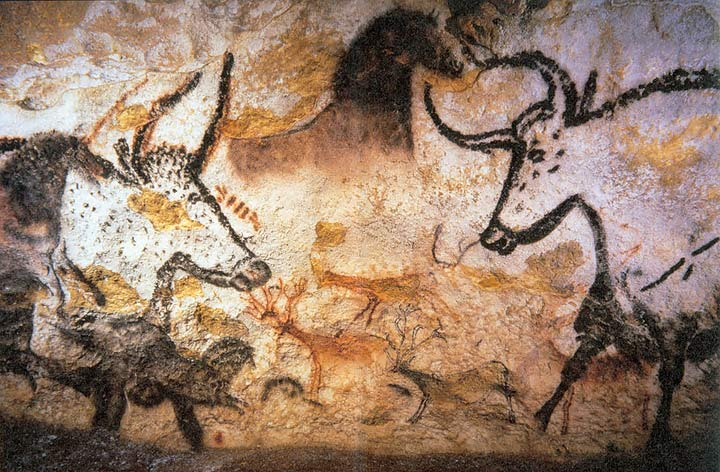
\includegraphics[width=4cm]{figures/1174006/1174006gua1.jpg}
	\centering
	\caption{Gua Lascaux.}
\end{figure}
Pada 35000 tahun yang lalu, di sebuah dinding tepatnya di gua Lascaux, Perancis, para pemburu Cro-Magnon menggambarkan hewan-hewan mangsa mereka. Mereka juga menggambarkan garis-garis yang dipercaya sebagai rute dari migrasi hewan-hewan mangsa mereka tersebut. Catatan awal tersebut sejalan dengan dua elemen struktur pada sistem informasi geografis modern saat ini, arsip grafis yang terhubung ke database atribut. 
Lalu pada tahun 1700-an teknik survei modern untuk pemetaan topografis diterapkan, termasuk versi awal pemetaan tematis, contohnya untuk keilmuan atau data sensus. 
Kemudian pada awal abad ke-20 memperlihatkan pengembangan "litografi foto" dimana peta dipisahkan menjadi beberapa lapisan (layer). Perkembangan perangkat keras komputer yang dipacu oleh penelitian senjata nuklir membawa aplikasi pemetaan menjadi multifungsi pada awal tahun 1960-an. 
Setelah itu, pada tahun 1967 menjadi awal pengembangan sistem informasi geografis yang bisa diterapkan di Ottawa, Ontario oleh Departemen Energi, Pertambangan dan Sumber Daya. Sistem ini dikembangkan oleh Roger Tomlinson, yang kemudian disebut CGIS (Canadian GIS - SIG Kanada) yang digunakan untuk menyimpan, menganalisis dan mengolah data-data yang sebelumnya telah dikumpulkan untuk kepentingan Inventarisasi Tanah di Kanada (CLI - Canadian land Inventory) - dimana ini merupakan sebuah inisiatif untuk mengetahui kemampuan dari suatu lahan yang ada di wilayah pedesaan Kanada dengan cara memetakaan berbagai informasi mengenai tanah, pertanian, pariwisata, alam bebas, unggas dan penggunaan tanah pada skala 1:250000. Faktor pemeringkatan klasifikasi juga diterapkan untuk keperluan analisis.
\begin{figure}[H]
	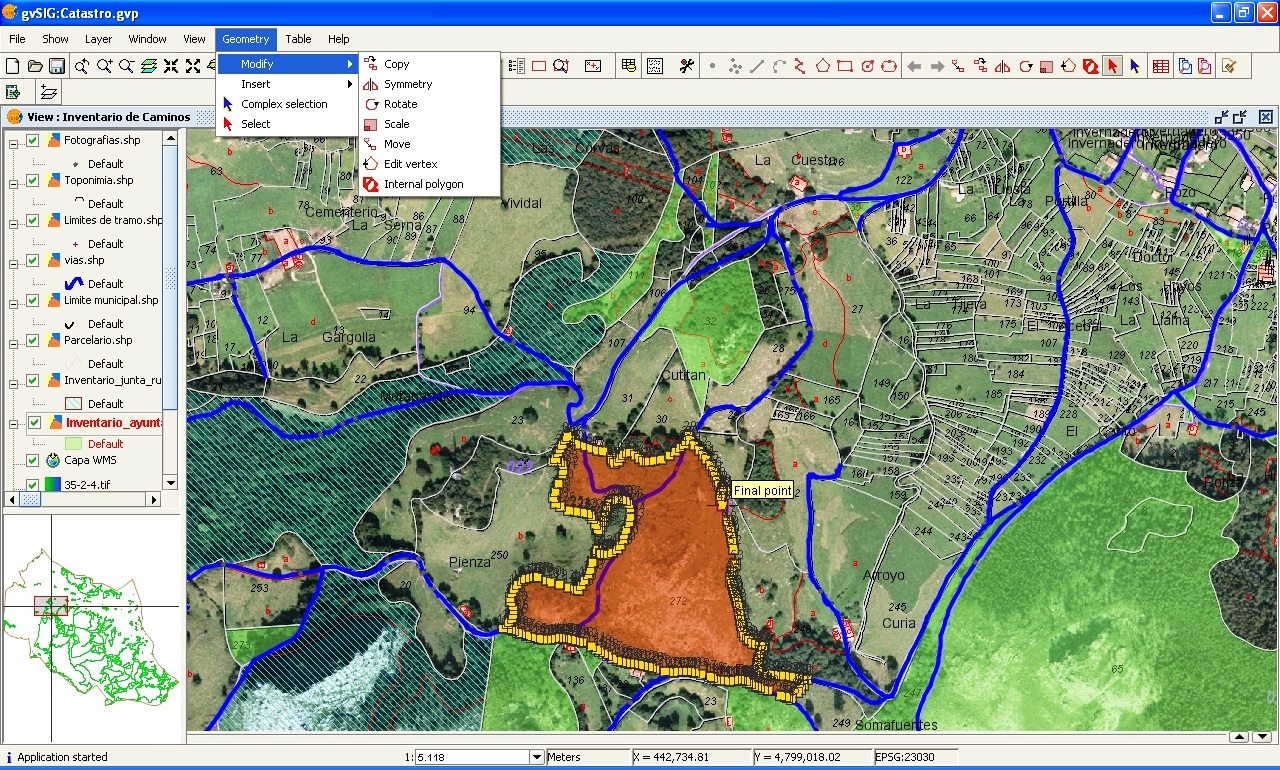
\includegraphics[width=4cm]{figures/1174006/1174006sigapp1.jpg}
	\centering
	\caption{Aplikasi SIG.}
\end{figure}
\subsection{Koordinat}
Koordinat digunakan untuk menunjukkan suatu titik di bumi berdasarkan garis lintang dan garis bujur. Koordinat dibagi menjadi dua bagian irisan yaitu irisan melintang yang disebut dengan garis lintang mulai dari khatulistiwa, membesar ke arah kutub(utara mupun selatan) sedangkanyang lain membujur mulai dari garis Greenwhich membesar ke arah barat dan timur. Satuan skala pada koordinat dibagi menjadi derajat lintang 0\textdegree sampai 90\textdegree dan bujur 0\textdegree sampai 180\textdegree.
Informasi sebuah lokasi didasarkan pada sistem koordinat, yang mencakup datum dan proyeksi peta. Datum adalah kumpulan parameter dan titik kontrol yanghubungan geometriknya diketahui, baik melalui pengukuranatau penghitungan. Sedangkan sistem proyeksi peta adalah sistem yang dirancang untuk merepresentasikan permukaan dari suatu bidang lengkung atau spheroid (misalnya bumi) pada suatu bidang datar. Proses representasi ini menyebabkan distorsi yang perlu diperhitungkan untuk memperoleh ketelitian beberapa macam properti, seperti jarak, sudut, atau luasan.
\begin{figure}[H]
	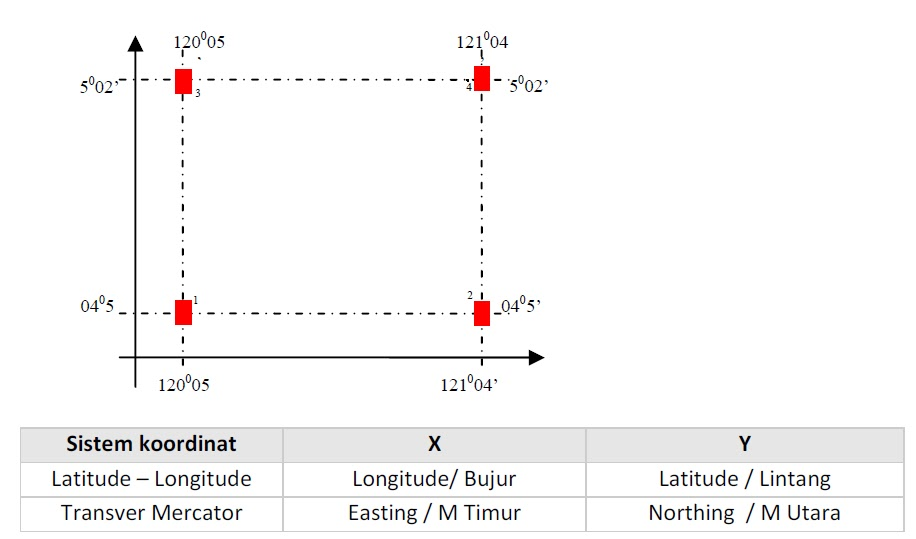
\includegraphics[width=4cm]{figures/1174006/1174006koordinat1.jpg}
	\centering
	\caption{Sistem Koordinat.}
\end{figure}
\subsection{Data Geospasial}
\subsubsection{Data Vektor}
Data vektor adalah data yang direkam dalam bentuk koordinat titik yang menampilkan, menempatkan, dan menyimpan data spasial dengan menggunakan titik, garis atau area (polygon).
\begin{figure}[H]
	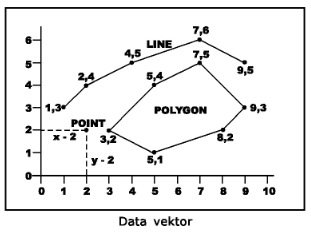
\includegraphics[width=4cm]{figures/1174006/1174006vektor1.png}
	\centering
	\caption{Data Vektor.}
\end{figure}
Ada tipe-tipe data vector yang bisa digunakan untuk menampilkan informasi pada peta. 
\begin{enumerate}
	\item Titik bisa digunakan sebagai lokasi sebuah kota atau posisi tower radio. 
	\item Garis bisa digunakan untuk menunjukkan route suatu perjalanan atau menggambarkan boundary.
	\item Poligon bisa digunakan untuk menggambarkan sebuah danau atau sebuah Negara pada peta dunia.
\end{enumerate}

\subsubsection{Data Raster}
Data raster adalah data yang disimpan dalam bentuk grid atau petak sehingga terbentuk suatu ruang yang teratur dalam bentuk pixel. 
Foto digital seperti areal fotografi atau satelit merupakan bagian dari data raster pada peta.
\begin{figure}[H]
	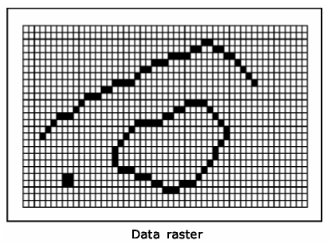
\includegraphics[width=4cm]{figures/1174006/1174006raster1.png}
	\centering
	\caption{Data Raster.}
\end{figure}
Data raster dihasilkan dari sistem penginderaan jauh dan sangat baik untuk merepresentasikan batas-batas yang berubah secara gradual seperti jenis tanah, kelembaban tanah, suhu, dan lain-lain.
Obyek geografis pada data rastel direpresentasikan sebagai struktur sel grid yang disebut sebagai pixel.
Resolusi tergantung pada ukuran pixelnya, semakin kecil ukuran permukaan bumi yang direpresentasikan oleh sel, semakin tinggi resolusinya. Dengan kata lain, resolusi pixel menggambarkan ukuran sebenarnya dipermukaan bumi yang diwakili oleh setiap pixel pada citra.

\subsubsection{Perbedaan Data Vektor dan Data Rastel}
Data vektor relatif lebih ekonomis dalam hal ukuran file dan presisi dalam lokasi. Tetapi sangat sulit untuk digunakan dalam komputasi matematik. Sebaliknya data raster biasanya membutuhkan ruang penyimpanan file yang lebih besar dan presisi lokasinya lebih rendah tetapi lebih mudah digunakan secara matematis.

\subsection{Link}
\href{link kamu}{alias}

\subsection{Plagiarism}
\begin{figure}[H]
	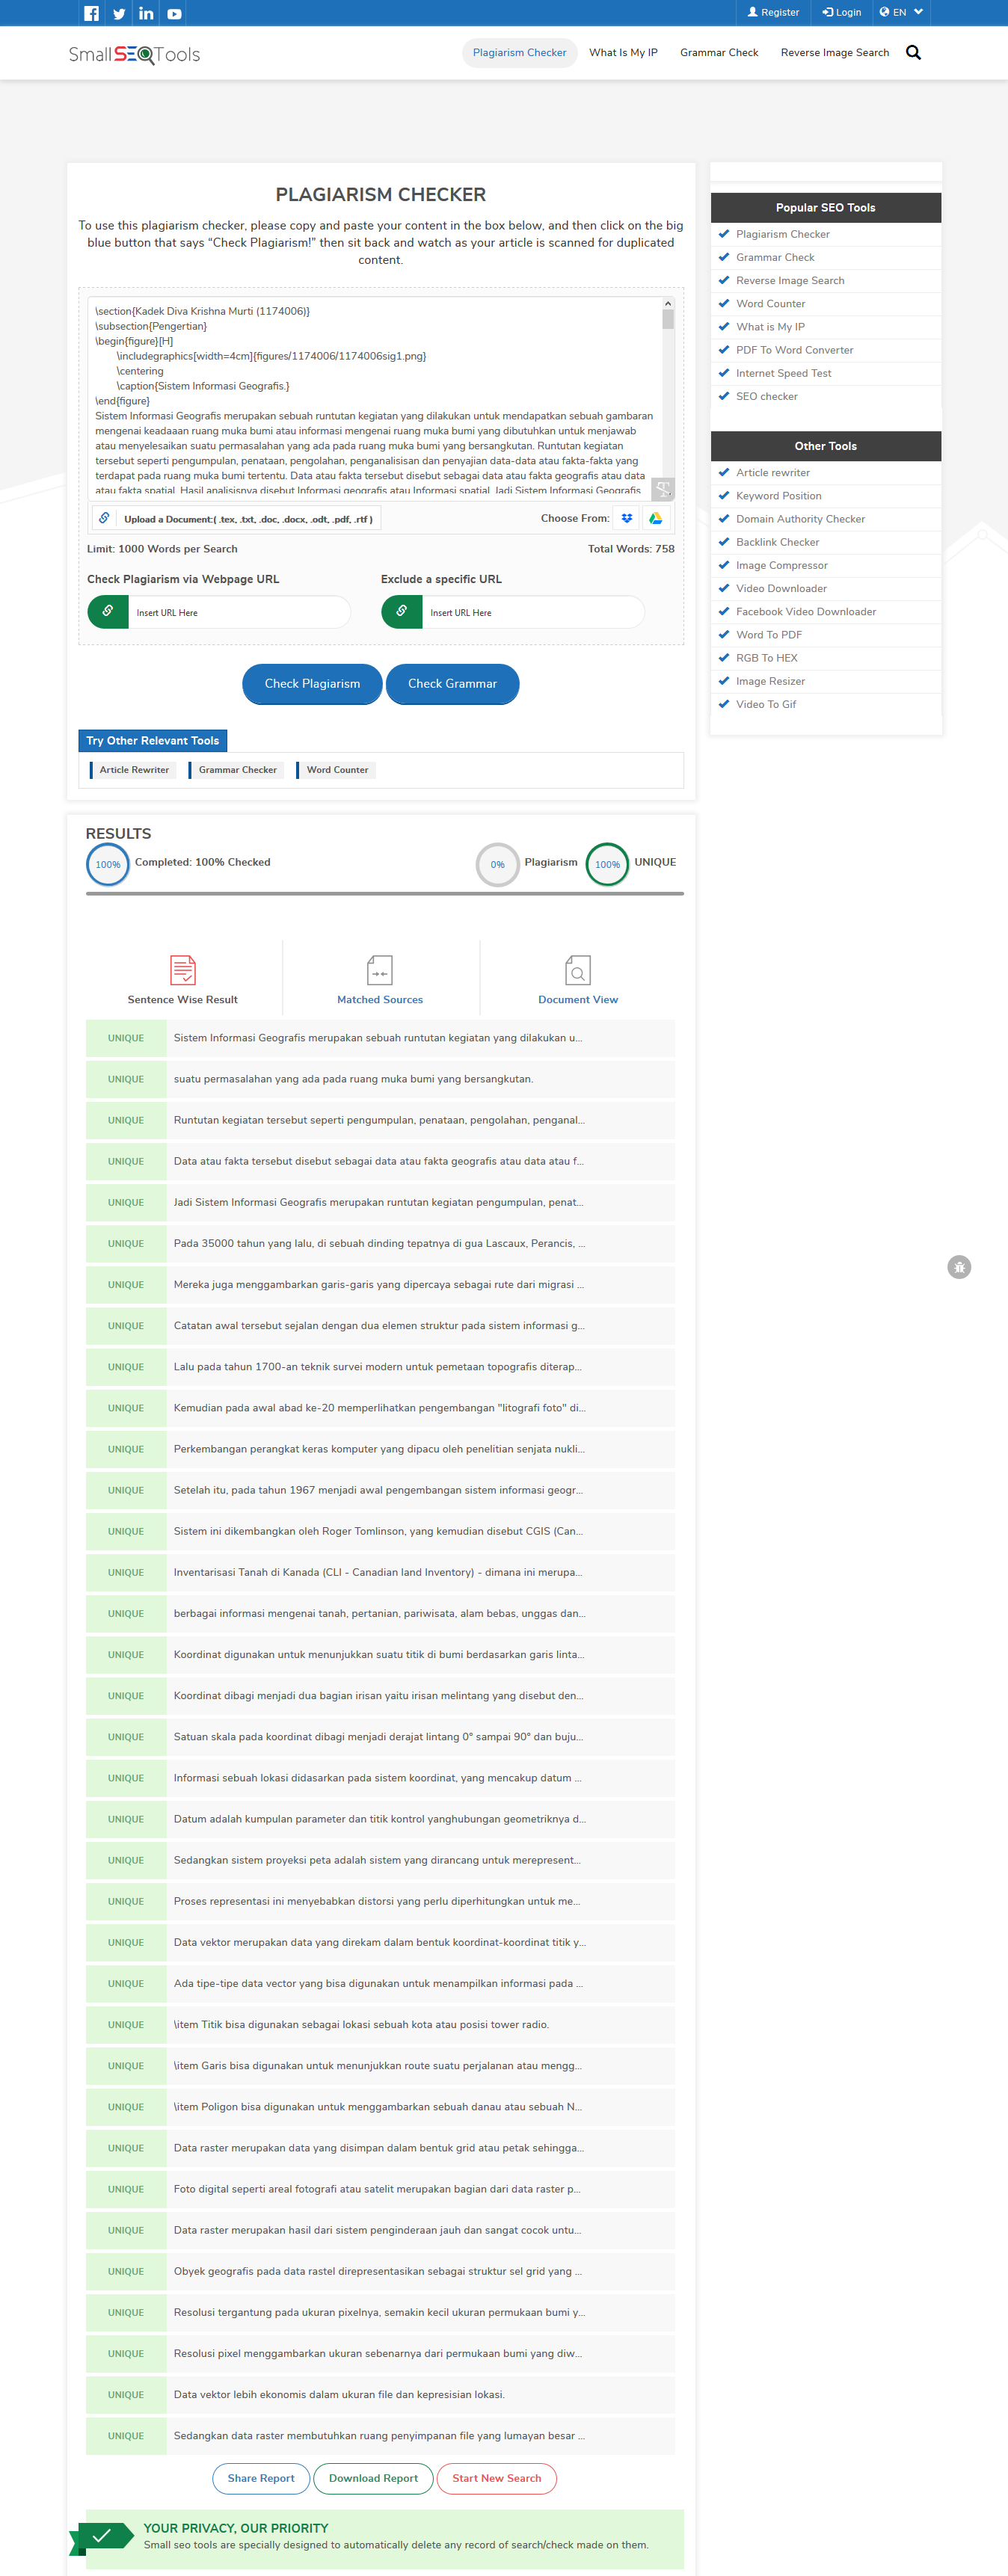
\includegraphics[width=4cm]{figures/1174006/1174006plagiarism1.png}
	\centering
	\caption{Plagiarism 1174006.}
\end{figure}

\section{NAMA (NPM)}
\subsection{Pengertian}
\subsection{Sejarah}
\subsection{Koordinat}
\subsection{Data Geospasial}
\subsection{Link}
\subsection{Plagiarism}

\subsection{Cara Penggunaan}
\subsubsection{Gambar}

\hfill\break

Contoh Gambar
\begin{figure}[H]
	
\includegraphics[width=4cm]{figures/himatif.png}
	\centering
	\caption{Contoh gambar.}
\end{figure}

\subsubsection{List}
\begin{enumerate}
	\item Satu
	\item Dua
\end{enumerate}

\begin{itemize}
	\item Satu
	\item Dua
\end{itemize}

\href{link kamu}{alias}
contoh link
\href{https://www.google.com/}{klik me}
\section{NAMA (NPM)}
\subsection{Pengertian}
\subsection{Sejarah}
\subsection{Koordinat}
\subsection{Data Geospasial}
\subsection{Link}
\subsection{Plagiarism}

\subsection{Cara Penggunaan}
\subsubsection{Gambar}

\hfill\break

Contoh Gambar
\begin{figure}[H]
	
\includegraphics[width=4cm]{figures/himatif.png}
	\centering
	\caption{Contoh gambar.}
\end{figure}

\subsubsection{List}
\begin{enumerate}
	\item Satu
	\item Dua
\end{enumerate}

\begin{itemize}
	\item Satu
	\item Dua
\end{itemize}

\href{link kamu}{alias}
contoh link
\href{https://www.google.com/}{klik me}
\section{NAMA (NPM)}
\subsection{Pengertian}
\subsection{Sejarah}
\subsection{Koordinat}
\subsection{Data Geospasial}
\subsection{Link}
\subsection{Plagiarism}

\subsection{Cara Penggunaan}
\subsubsection{Gambar}

\hfill\break

Contoh Gambar
\begin{figure}[H]
	
\includegraphics[width=4cm]{figures/himatif.png}
	\centering
	\caption{Contoh gambar.}
\end{figure}

\subsubsection{List}
\begin{enumerate}
	\item Satu
	\item Dua
\end{enumerate}

\begin{itemize}
	\item Satu
	\item Dua
\end{itemize}

\href{link kamu}{alias}
contoh link
\href{https://www.google.com/}{klik me}
\section{NAMA (NPM)}
\subsection{Pengertian}
\subsection{Sejarah}
\subsection{Koordinat}
\subsection{Data Geospasial}
\subsection{Link}
\subsection{Plagiarism}

\subsection{Cara Penggunaan}
\subsubsection{Gambar}

\hfill\break

Contoh Gambar
\begin{figure}[H]
	
\includegraphics[width=4cm]{figures/himatif.png}
	\centering
	\caption{Contoh gambar.}
\end{figure}

\subsubsection{List}
\begin{enumerate}
	\item Satu
	\item Dua
\end{enumerate}

\begin{itemize}
	\item Satu
	\item Dua
\end{itemize}

\href{link kamu}{alias}
contoh link
\href{https://www.google.com/}{klik me}
\section{NAMA (NPM)}
\subsection{Pengertian}
\subsection{Sejarah}
\subsection{Koordinat}
\subsection{Data Geospasial}
\subsection{Link}
\subsection{Plagiarism}

\subsection{Cara Penggunaan}
\subsubsection{Gambar}

\hfill\break

Contoh Gambar
\begin{figure}[H]
	
\includegraphics[width=4cm]{figures/himatif.png}
	\centering
	\caption{Contoh gambar.}
\end{figure}

\subsubsection{List}
\begin{enumerate}
	\item Satu
	\item Dua
\end{enumerate}

\begin{itemize}
	\item Satu
	\item Dua
\end{itemize}

\href{link kamu}{alias}
contoh link
\href{https://www.google.com/}{klik me}
\section{NAMA (NPM)}
\subsection{Pengertian}
\subsection{Sejarah}
\subsection{Koordinat}
\subsection{Data Geospasial}
\subsection{Link}
\subsection{Plagiarism}

\subsection{Cara Penggunaan}
\subsubsection{Gambar}

\hfill\break

Contoh Gambar
\begin{figure}[H]
	
\includegraphics[width=4cm]{figures/himatif.png}
	\centering
	\caption{Contoh gambar.}
\end{figure}

\subsubsection{List}
\begin{enumerate}
	\item Satu
	\item Dua
\end{enumerate}

\begin{itemize}
	\item Satu
	\item Dua
\end{itemize}

\href{link kamu}{alias}
contoh link
\href{https://www.google.com/}{klik me}
\section{NAMA (NPM)}
\subsection{Pengertian}
\subsection{Sejarah}
\subsection{Koordinat}
\subsection{Data Geospasial}
\subsection{Link}
\subsection{Plagiarism}

\subsection{Cara Penggunaan}
\subsubsection{Gambar}

\hfill\break

Contoh Gambar
\begin{figure}[H]
	
\includegraphics[width=4cm]{figures/himatif.png}
	\centering
	\caption{Contoh gambar.}
\end{figure}

\subsubsection{List}
\begin{enumerate}
	\item Satu
	\item Dua
\end{enumerate}

\begin{itemize}
	\item Satu
	\item Dua
\end{itemize}

\href{link kamu}{alias}
contoh link
\href{https://www.google.com/}{klik me}
\section{NAMA (NPM)}
\subsection{Pengertian}
\subsection{Sejarah}
\subsection{Koordinat}
\subsection{Data Geospasial}
\subsection{Link}
\subsection{Plagiarism}

\subsection{Cara Penggunaan}
\subsubsection{Gambar}

\hfill\break

Contoh Gambar
\begin{figure}[H]
	
\includegraphics[width=4cm]{figures/himatif.png}
	\centering
	\caption{Contoh gambar.}
\end{figure}

\subsubsection{List}
\begin{enumerate}
	\item Satu
	\item Dua
\end{enumerate}

\begin{itemize}
	\item Satu
	\item Dua
\end{itemize}

\href{link kamu}{alias}
contoh link
\href{https://www.google.com/}{klik me}
\section{NAMA (NPM)}
\subsection{Pengertian}
\subsection{Sejarah}
\subsection{Koordinat}
\subsection{Data Geospasial}
\subsection{Link}
\subsection{Plagiarism}

\subsection{Cara Penggunaan}
\subsubsection{Gambar}

\hfill\break

Contoh Gambar
\begin{figure}[H]
	
\includegraphics[width=4cm]{figures/himatif.png}
	\centering
	\caption{Contoh gambar.}
\end{figure}

\subsubsection{List}
\begin{enumerate}
	\item Satu
	\item Dua
\end{enumerate}

\begin{itemize}
	\item Satu
	\item Dua
\end{itemize}

\href{link kamu}{alias}
contoh link
\href{https://www.google.com/}{klik me}
%\chapter{Tugas Kedua}
%\section{NAMA (NPM)}
\subsection{Pengertian}
\subsection{Sejarah}
\subsection{Koordinat}
\subsection{Data Geospasial}
\subsection{Link}
\subsection{Plagiarism}

\subsection{Cara Penggunaan}
\subsubsection{Gambar}

\hfill\break

Contoh Gambar
\begin{figure}[H]
	
\includegraphics[width=4cm]{figures/himatif.png}
	\centering
	\caption{Contoh gambar.}
\end{figure}

\subsubsection{List}
\begin{enumerate}
	\item Satu
	\item Dua
\end{enumerate}

\begin{itemize}
	\item Satu
	\item Dua
\end{itemize}

\href{link kamu}{alias}
contoh link
\href{https://www.google.com/}{klik me}
%\section{NAMA (NPM)}
\subsection{Pengertian}
\subsection{Sejarah}
\subsection{Koordinat}
\subsection{Data Geospasial}
\subsection{Link}
\subsection{Plagiarism}

\subsection{Cara Penggunaan}
\subsubsection{Gambar}

\hfill\break

Contoh Gambar
\begin{figure}[H]
	
\includegraphics[width=4cm]{figures/himatif.png}
	\centering
	\caption{Contoh gambar.}
\end{figure}

\subsubsection{List}
\begin{enumerate}
	\item Satu
	\item Dua
\end{enumerate}

\begin{itemize}
	\item Satu
	\item Dua
\end{itemize}

\href{link kamu}{alias}
contoh link
\href{https://www.google.com/}{klik me}
%\section{NAMA (NPM)}
\subsection{Pengertian}
\subsection{Sejarah}
\subsection{Koordinat}
\subsection{Data Geospasial}
\subsection{Link}
\subsection{Plagiarism}

\subsection{Cara Penggunaan}
\subsubsection{Gambar}

\hfill\break

Contoh Gambar
\begin{figure}[H]
	
\includegraphics[width=4cm]{figures/himatif.png}
	\centering
	\caption{Contoh gambar.}
\end{figure}

\subsubsection{List}
\begin{enumerate}
	\item Satu
	\item Dua
\end{enumerate}

\begin{itemize}
	\item Satu
	\item Dua
\end{itemize}

\href{link kamu}{alias}
contoh link
\href{https://www.google.com/}{klik me}

%\section{NAMA (NPM)}
\subsection{Pengertian}
\subsection{Sejarah}
\subsection{Koordinat}
\subsection{Data Geospasial}
\subsection{Link}
\subsection{Plagiarism}

\subsection{Cara Penggunaan}
\subsubsection{Gambar}

\hfill\break

Contoh Gambar
\begin{figure}[H]
	
\includegraphics[width=4cm]{figures/himatif.png}
	\centering
	\caption{Contoh gambar.}
\end{figure}

\subsubsection{List}
\begin{enumerate}
	\item Satu
	\item Dua
\end{enumerate}

\begin{itemize}
	\item Satu
	\item Dua
\end{itemize}

\href{link kamu}{alias}
contoh link
\href{https://www.google.com/}{klik me}
%\section{NAMA (NPM)}
\subsection{Pengertian}
\subsection{Sejarah}
\subsection{Koordinat}
\subsection{Data Geospasial}
\subsection{Link}
\subsection{Plagiarism}

\subsection{Cara Penggunaan}
\subsubsection{Gambar}

\hfill\break

Contoh Gambar
\begin{figure}[H]
	
\includegraphics[width=4cm]{figures/himatif.png}
	\centering
	\caption{Contoh gambar.}
\end{figure}

\subsubsection{List}
\begin{enumerate}
	\item Satu
	\item Dua
\end{enumerate}

\begin{itemize}
	\item Satu
	\item Dua
\end{itemize}

\href{link kamu}{alias}
contoh link
\href{https://www.google.com/}{klik me}
%\section{NAMA (NPM)}
\subsection{Pengertian}
\subsection{Sejarah}
\subsection{Koordinat}
\subsection{Data Geospasial}
\subsection{Link}
\subsection{Plagiarism}

\subsection{Cara Penggunaan}
\subsubsection{Gambar}

\hfill\break

Contoh Gambar
\begin{figure}[H]
	
\includegraphics[width=4cm]{figures/himatif.png}
	\centering
	\caption{Contoh gambar.}
\end{figure}

\subsubsection{List}
\begin{enumerate}
	\item Satu
	\item Dua
\end{enumerate}

\begin{itemize}
	\item Satu
	\item Dua
\end{itemize}

\href{link kamu}{alias}
contoh link
\href{https://www.google.com/}{klik me}
%\section{NAMA (NPM)}
\subsection{Pengertian}
\subsection{Sejarah}
\subsection{Koordinat}
\subsection{Data Geospasial}
\subsection{Link}
\subsection{Plagiarism}

\subsection{Cara Penggunaan}
\subsubsection{Gambar}

\hfill\break

Contoh Gambar
\begin{figure}[H]
	
\includegraphics[width=4cm]{figures/himatif.png}
	\centering
	\caption{Contoh gambar.}
\end{figure}

\subsubsection{List}
\begin{enumerate}
	\item Satu
	\item Dua
\end{enumerate}

\begin{itemize}
	\item Satu
	\item Dua
\end{itemize}

\href{link kamu}{alias}
contoh link
\href{https://www.google.com/}{klik me}
%\section{NAMA (NPM)}
\subsection{Pengertian}
\subsection{Sejarah}
\subsection{Koordinat}
\subsection{Data Geospasial}
\subsection{Link}
\subsection{Plagiarism}

\subsection{Cara Penggunaan}
\subsubsection{Gambar}

\hfill\break

Contoh Gambar
\begin{figure}[H]
	
\includegraphics[width=4cm]{figures/himatif.png}
	\centering
	\caption{Contoh gambar.}
\end{figure}

\subsubsection{List}
\begin{enumerate}
	\item Satu
	\item Dua
\end{enumerate}

\begin{itemize}
	\item Satu
	\item Dua
\end{itemize}

\href{link kamu}{alias}
contoh link
\href{https://www.google.com/}{klik me}
%\section{NAMA (NPM)}
\subsection{Pengertian}
\subsection{Sejarah}
\subsection{Koordinat}
\subsection{Data Geospasial}
\subsection{Link}
\subsection{Plagiarism}

\subsection{Cara Penggunaan}
\subsubsection{Gambar}

\hfill\break

Contoh Gambar
\begin{figure}[H]
	
\includegraphics[width=4cm]{figures/himatif.png}
	\centering
	\caption{Contoh gambar.}
\end{figure}

\subsubsection{List}
\begin{enumerate}
	\item Satu
	\item Dua
\end{enumerate}

\begin{itemize}
	\item Satu
	\item Dua
\end{itemize}

\href{link kamu}{alias}
contoh link
\href{https://www.google.com/}{klik me}
%\section{NAMA (NPM)}
\subsection{Pengertian}
\subsection{Sejarah}
\subsection{Koordinat}
\subsection{Data Geospasial}
\subsection{Link}
\subsection{Plagiarism}

\subsection{Cara Penggunaan}
\subsubsection{Gambar}

\hfill\break

Contoh Gambar
\begin{figure}[H]
	
\includegraphics[width=4cm]{figures/himatif.png}
	\centering
	\caption{Contoh gambar.}
\end{figure}

\subsubsection{List}
\begin{enumerate}
	\item Satu
	\item Dua
\end{enumerate}

\begin{itemize}
	\item Satu
	\item Dua
\end{itemize}

\href{link kamu}{alias}
contoh link
\href{https://www.google.com/}{klik me}
%\section{NAMA (NPM)}
\subsection{Pengertian}
\subsection{Sejarah}
\subsection{Koordinat}
\subsection{Data Geospasial}
\subsection{Link}
\subsection{Plagiarism}

\subsection{Cara Penggunaan}
\subsubsection{Gambar}

\hfill\break

Contoh Gambar
\begin{figure}[H]
	\includegraphics[width=4cm]{figures/himatif.png}
	\centering
	\caption{Contoh gambar.}
\end{figure}

\subsubsection{List}
\begin{enumerate}
	\item Satu
	\item Dua
\end{enumerate}

\begin{itemize}
	\item Satu
	\item Dua
\end{itemize}

\href{link kamu}{alias}
contoh link
\href{https://www.google.com/}{klik me}
%\section{NAMA (NPM)}
\subsection{Pengertian}
\subsection{Sejarah}
\subsection{Koordinat}
\subsection{Data Geospasial}
\subsection{Link}
\subsection{Plagiarism}

\subsection{Cara Penggunaan}
\subsubsection{Gambar}

\hfill\break

Contoh Gambar
\begin{figure}[H]
	\includegraphics[width=4cm]{figures/himatif.png}
	\centering
	\caption{Contoh gambar.}
\end{figure}

\subsubsection{List}
\begin{enumerate}
	\item Satu
	\item Dua
\end{enumerate}

\begin{itemize}
	\item Satu
	\item Dua
\end{itemize}

\href{link kamu}{alias}
contoh link
\href{https://www.google.com/}{klik me}
%\section{NAMA (NPM)}
\subsection{Pengertian}
\subsection{Sejarah}
\subsection{Koordinat}
\subsection{Data Geospasial}
\subsection{Link}
\subsection{Plagiarism}

\subsection{Cara Penggunaan}
\subsubsection{Gambar}

\hfill\break

Contoh Gambar
\begin{figure}[H]
	\includegraphics[width=4cm]{figures/himatif.png}
	\centering
	\caption{Contoh gambar.}
\end{figure}

\subsubsection{List}
\begin{enumerate}
	\item Satu
	\item Dua
\end{enumerate}

\begin{itemize}
	\item Satu
	\item Dua
\end{itemize}

\href{link kamu}{alias}
contoh link
\href{https://www.google.com/}{klik me}
%\section{NAMA (NPM)}
\subsection{Pengertian}
\subsection{Sejarah}
\subsection{Koordinat}
\subsection{Data Geospasial}
\subsection{Link}
\subsection{Plagiarism}

\subsection{Cara Penggunaan}
\subsubsection{Gambar}

\hfill\break

Contoh Gambar
\begin{figure}[H]
	\includegraphics[width=4cm]{figures/himatif.png}
	\centering
	\caption{Contoh gambar.}
\end{figure}

\subsubsection{List}
\begin{enumerate}
	\item Satu
	\item Dua
\end{enumerate}

\begin{itemize}
	\item Satu
	\item Dua
\end{itemize}

\href{link kamu}{alias}
contoh link
\href{https://www.google.com/}{klik me}
%\section{NAMA (NPM)}
\subsection{Pengertian}
\subsection{Sejarah}
\subsection{Koordinat}
\subsection{Data Geospasial}
\subsection{Link}
\subsection{Plagiarism}

\subsection{Cara Penggunaan}
\subsubsection{Gambar}

\hfill\break

Contoh Gambar
\begin{figure}[H]
	\includegraphics[width=4cm]{figures/himatif.png}
	\centering
	\caption{Contoh gambar.}
\end{figure}

\subsubsection{List}
\begin{enumerate}
	\item Satu
	\item Dua
\end{enumerate}

\begin{itemize}
	\item Satu
	\item Dua
\end{itemize}

\href{link kamu}{alias}
contoh link
\href{https://www.google.com/}{klik me}
%\section{NAMA (NPM)}
\subsection{Pengertian}
\subsection{Sejarah}
\subsection{Koordinat}
\subsection{Data Geospasial}
\subsection{Link}
\subsection{Plagiarism}

\subsection{Cara Penggunaan}
\subsubsection{Gambar}

\hfill\break

Contoh Gambar
\begin{figure}[H]
	\includegraphics[width=4cm]{figures/himatif.png}
	\centering
	\caption{Contoh gambar.}
\end{figure}

\subsubsection{List}
\begin{enumerate}
	\item Satu
	\item Dua
\end{enumerate}

\begin{itemize}
	\item Satu
	\item Dua
\end{itemize}

\href{link kamu}{alias}
contoh link
\href{https://www.google.com/}{klik me}
%\section{NAMA (NPM)}
\subsection{Pengertian}
\subsection{Sejarah}
\subsection{Koordinat}
\subsection{Data Geospasial}
\subsection{Link}
\subsection{Plagiarism}

\subsection{Cara Penggunaan}
\subsubsection{Gambar}

\hfill\break

Contoh Gambar
\begin{figure}[H]
	\includegraphics[width=4cm]{figures/himatif.png}
	\centering
	\caption{Contoh gambar.}
\end{figure}

\subsubsection{List}
\begin{enumerate}
	\item Satu
	\item Dua
\end{enumerate}

\begin{itemize}
	\item Satu
	\item Dua
\end{itemize}

\href{link kamu}{alias}
contoh link
\href{https://www.google.com/}{klik me}
%\section{NAMA (NPM)}
\subsection{Pengertian}
\subsection{Sejarah}
\subsection{Koordinat}
\subsection{Data Geospasial}
\subsection{Link}
\subsection{Plagiarism}

\subsection{Cara Penggunaan}
\subsubsection{Gambar}

\hfill\break

Contoh Gambar
\begin{figure}[H]
	\includegraphics[width=4cm]{figures/himatif.png}
	\centering
	\caption{Contoh gambar.}
\end{figure}

\subsubsection{List}
\begin{enumerate}
	\item Satu
	\item Dua
\end{enumerate}

\begin{itemize}
	\item Satu
	\item Dua
\end{itemize}

\href{link kamu}{alias}
contoh link
\href{https://www.google.com/}{klik me}
\bibliographystyle{IEEEtran}
%\def\bibfont{\normalsize}
\bibliography{references}
%%%%%%%%%%%%%%%%%%%%%%%%%%%%%%%%%%%%%%%%%%%%%%


%%%%%%%%%%%%%%%
%%  The default LaTeX Index
%%  Don't need to add any commands before \begin{document}
\printindex

%%%% Making an index
%%
%% 1. Make index entries, don't leave any spaces so that they
%% will be sorted correctly.
%%
%% \index{term}
%% \index{term!subterm}
%% \index{term!subterm!subsubterm}
%%
%% 2. Run LaTeX several times to produce <filename>.idx
%%
%% 3. On command line, type  makeindx <filename> which
%% will produce <filename>.ind
%%
%% 4. Type \printindex to make the index appear in your book.
%%
%% 5. If you would like to edit <filename>.ind
%% you may do so. See docs.pdf for more information.
%%
%%%%%%%%%%%%%%%%%%%%%%%%%%%%%%

%%%%%%%%%%%%%% Making Multiple Indices %%%%%%%%%%%%%%%%
%% 1.
%% \usepackage{multind}
%% \makeindex{book}
%% \makeindex{authors}
%% \begin{document}
%%
%% 2.
%% % add index terms to your book, ie,
%% \index{book}{A term to go to the topic index}
%% \index{authors}{Put this author in the author index}
%%
%% \index{book}{Cows}
%% \index{book}{Cows!Jersey}
%% \index{book}{Cows!Jersey!Brown}
%%
%% \index{author}{Douglas Adams}
%% \index{author}{Boethius}
%% \index{author}{Mark Twain}
%%
%% 3. On command line type
%% makeindex topic
%% makeindex authors
%%
%% 4.
%% this is a Wiley command to make the indices print:
%% \multiprintindex{book}{Topic index}
%% \multiprintindex{authors}{Author index}

\end{document}

